\documentclass[10pt]{book}
\author{Lan Peng, PhD Student\\ \\Department of Industrial and Systems Engineering\\University at Buffalo, SUNY\\lanpeng@buffalo.edu}
\title{Notes for Operations Research \& More}

\usepackage{amsmath}
\usepackage{amssymb}
\usepackage{amsthm}
\usepackage{color}
\usepackage{tabularx}
\usepackage{algorithm}
\usepackage{algorithmic}
\usepackage{bm}
\usepackage{mathrsfs}
\usepackage{hyperref}
\usepackage{longtable}
\usepackage{makecell}
\usepackage{lscape}

\usepackage[
	letterpaper,
	left=2cm,
	right=2cm,
	top=2cm,
	bottom=2cm]{geometry}

\usepackage{tikz}
	\usetikzlibrary{shapes.geometric, arrows}
	\usetikzlibrary{arrows,shapes,matrix}
	\usetikzlibrary{decorations.pathmorphing} 
	\usepgflibrary{plotmarks}
	\usetikzlibrary{patterns}  
	\usetikzlibrary{positioning} 
	\tikzstyle{roundedRectangle} = [rectangle, rounded corners, minimum width=3cm, minimum height=1cm,text centered, draw=black]
	\tikzstyle{io} = [trapezium, trapezium left angle=70, trapezium right angle=110, minimum width=3cm, minimum height=1cm, text centered, draw=black]
	\tikzstyle{process} = [rectangle, minimum width=2cm, minimum height=1cm, text centered, draw=black, inner sep=0.1cm]
	\tikzstyle{decision} = [diamond, minimum width=2cm, minimum height=0cm, text centered, draw=black, inner sep=0cm]
	\tikzstyle{arrow} = [thick,->,>=stealth]
	\tikzstyle{link} = [thick, -]
	\tikzstyle{circleNode} = [circle, minimum size = 1cm, text centered, draw=black, inner sep=0.1cm]

\newtheorem{definition}{Definition}[section]
\newtheorem*{remark}{Remark}
\newtheorem{theorem}{Theorem}[section]
\newtheorem{corollary}{Corollary}[theorem]
\newtheorem{lemma}[theorem]{Lemma}

\newcommand{\todo}[1]{
	\vspace{5 mm}
	\par
	\noindent
	\marginpar{\textsc{to do}}
	\framebox{
		\begin{minipage}[c]{0.95 \textwidth}
		\tt
		\begin{center} 
			#1
		\end{center}
		\end{minipage}
	}
	\vspace{5 mm}
	\par
}

% \newcommand{\definition}[1]{
% 	\vspace{5 mm}
% 	\par
% 	\noindent
% 	\colorbox{cyan!10}{
% 		\begin{minipage}[c]{0.95 \textwidth}
% 			\textbf{\color{blue}Definition:}~#1
% 		\end{minipage}
% 	}
% 	\vspace{5 mm}
% 	\par
% }

\newcommand{\alert}[1]{
	{\color{red}#1}
}

\newcommand{\edited}[1]{{\color{blue}#1}}

\newcommand{\fixme}[1]{{\color{red}#1}\marginpar{\textsc{\color{red}fixme}}}

\newcommand{\note}[2][]{{\color{blue}#1	[\textsc{note}:~#2]}}

\begin{document}
	\maketitle
	\today
	\tableofcontents
	\part{Preliminary Topics}
	\chapter{Introduction to Optimization}

	\chapter{Review of Linear Algebra}
		\section{Field}
			\begin{definition}[Field]
				Let $F$ denote either the set  of real numbers or the set of complex numbers.
				\begin{itemize}
					\item Addition is commutative: $x + y = y + x, \forall x, y \in F$
					\item Addition is associative: $x + (y + z) = (x + y) + z, \forall x, y, z \in F$
					\item Element 0 exists and unique: $\exists 0, x + 0 = x, \forall x \in F$
					\item To each $x \in F$ there corresponds a unique element $(-x) \in F$ such that $x + (-x) = 0$
					\item Multiplication is commutative: $xy = yx, \forall x, y \in F$
					\item Multiplication is associative: $x(yz) = (xy)z, \forall x, y, z \in F$
					\item Element 1 exists and unique: $\exists 1, x1=x, \forall x \in F$
					\item To each $x\neq 0 \in F$ there corresponds a unique element $x^{-1} \in F$ that $xx^{-1} = 1$
					\item Multiplication distributes over addition: $x(y + z) = xy + xz, \forall x, y, z \in F$
				\end{itemize}
				Suppose one has a set $F$ of objects $x, y, z, ...$ and two operations on the elements of $F$ as follows. The first operation, called addition, associates with each pair of elements $x, y \in F$ an element $(x + y)\in F$; the second operation, called multiplication, associates with each pair $x, y$ an element $xy \in F$; and these two operations satisfy all conditions above. The set $F$, together with these two operations, is then called a \textbf{field}.
			\end{definition}

			\begin{definition}[Subfield]
				A \textbf{subfield} of the field $C$ is a set $F$ of complex numbers which itself is a field.
			\end{definition}

			\begin{example}
				The set of integers is not a field.
			\end{example}

			\begin{example}
				The set of rational numbers is a field.
			\end{example}

			\begin{example}
				The set of all complex numbers of the form $x + y\sqrt{2}$ where $x$ and $y$ are rational, is a subfield of $\mathbb{C}$.
			\end{example}

			\notice{In this note, we (...Lan) assume that the field involved is a subfield of the complex numbers $\mathbb{C}$. More generally, if $F$ is a field, it may be possible to add the unit $1$ to itself a finite number of times and obtain $0$, which does not happen in the subfield of $\mathbb{C}$. If it does happen in $F$, the least $n$ such that the sum of $n$ 1's is 0 is called \textbf{characteristic} of the field $F$. If it does not happen, then $F$ is called a field of \textbf{characteristic zero}.}

		\section{Real Vector Spaces}

		\section{Linear, Conic, Affine, and Convex Combinations}

		\section{Inner Products}
			\begin{definition}[Inner Product]
				Let $F$ be the field of real numbers or the field of complex numbers, and $V$ a vector space over $F$. An \textbf{inner product} on $V$ is a function which assigns to each ordered pair of vectors $\alpha$, $\beta$ in $V$ a scalar $<\alpha|\beta>$ in $F$ in such a way that $\forall \alpha, \beta, \gamma \in V, c \in \mathbb{R}$ that
				\begin{itemize}
					\item $<\alpha+\beta|\gamma> = <\alpha|\gamma> + <\beta|\gamma>$
					\item $<c\alpha|\beta> = c<\alpha|\beta>$
					\item $<\alpha|\beta> = \overline{<\beta|\alpha>}$
					\item $<\alpha|\alpha> \ge 0$, $<\alpha|\alpha> = 0$ iff $\alpha = \mathbf{0}$
				\end{itemize}
				Furthermore, the above properties imply that
				\begin{itemize}
					\item $<\alpha|c\beta+\gamma> = \bar{c}<\alpha|\beta> + <\alpha|\gamma>$
				\end{itemize}
			\end{definition}

			\begin{definition}
				On $F^n$ there is an inner product which we call the \textbf{standard inner product}. It is defined on $\mathbf{\alpha} = (x_1, x_2, ..., x_n)$ and $\mathbf{\beta} = (y_1, y_2, ..., y_n)$ by
				\begin{equation}
					<\alpha|\beta> = \sum_j x_j \bar{y_j}
				\end{equation}
				For $F = \mathbb{R}^n$
				\begin{equation}
					<\alpha|\beta> = \sum_j x_j y_j
				\end{equation}
				In the real case, the standard inner product is often called the dot product and denoted by $\alpha \cdot \beta$
			\end{definition}

			\begin{example}
				For $\mathbf{\alpha} = (x_1, x_2)$ and $\mathbf{\beta} = (y_1, y_2)$ in $\mathbb{R}^2$, the following is an inner product.
				\begin{equation}
					<\alpha|\beta> = x_1y_1 - x_2y_1 - x_1y_2 + 4x_2y_2
				\end{equation}
			\end{example}

			\begin{example}
				For $\mathbb{C}^{n\times n}$, 
				\begin{equation}
					<\mathbf{A}|\mathbf{B}> = trace(\mathbf{B}^* \mathbf{A})
				\end{equation}
				is an inner product, where
				\begin{equation}
					\mathbf{A}^*_{ij} = \bar{\mathbf{A}}_{ji} \quad (\textbf{conjugate transpose})
				\end{equation}
				For $\mathbb{R}^{n\times n}$,
				\begin{equation}
					<\mathbf{A}|\mathbf{B}> = trace(\mathbf{B}^T \mathbf{A}) = \sum_j (AB^T)_{jj} = \sum_j\sum_k A_{jk}B_{jk}
				\end{equation}
			\end{example}
			
		\section{Norms}

		\section{Eigenvectors and Eigenvalues}

		\section{}

	\chapter{Review of Real Analysis}
		\section{Sequences and Series}

		\section{Open Sets and Closed Sets}

	\part{Linear Programming}
	\chapter{Formulation}
		\section{Linear Programming Problem Manipulation}
			\subsection{Inequalities and Equalities}
				An inequality can be transformed into an equation by adding or subtracting the nonnegative slack or surplus variable
				\begin{equation}
					\sum_{j=1}^na_{ij}x_j \ge b_i \Rightarrow \sum_{j=1}^na_{ij}x_j - x_{n+1} = b_i 
				\end{equation}
				or
				\begin{equation}
					\sum_{j=1}^na_{ij}x_j \le b_i \Rightarrow \sum_{j=1}^na_{ij}x_j + x_{n+1} = b_i 
				\end{equation}
				Although it is not the practice, equality can be transformed into inequality too
				\begin{equation}
					\sum_{j=1}^na_{ij}x_j = b_i \Rightarrow \begin{cases}\sum_{j=1}^na_{ij}x_j \le b_i \\ \sum_{j=1}^na_{ij}x_j \ge b_i \end{cases} 
				\end{equation}
				Also, in linear programming, we only care about close set, so we will not have $<$, $>$ in the formulation, we can use the following
				\begin{equation}
					\sum_{j=1}^na_{ij}x_j > b_i \Rightarrow \sum_{j=1}^na_{ij}x_j \ge b_i + \epsilon 
				\end{equation}
				where $\epsilon$ is a small number.
			
			\subsection{Minimization and Maximization}
				To convert a minimization problem into a maximization problem, we can use the following to define a new objective function
				\begin{equation}
					\min \sum_{j=1}^nc_jx_j = -\max \sum_{j=1}^n c_jx_j 
				\end{equation}
			
			\subsection{Standard Form and Canonical Form}
				Standard Form
				\begin{align}
					\min \quad & \sum_{j=1}^nc_jx_j \\
					\text{s.t.} \quad & Ax = b \\
									  & x \ge 0 
				\end{align}
				Canonical Form
				\begin{align}
					\min \quad & \sum_{j=1}^nc_jx_j \\
					\text{s.t.} \quad & Ax \le b \\
									  & x \ge 0 
				\end{align}

		\section{Typical Problems}

		\section{Formulation Skills}
			\subsection{Absolute Value}
				Consider the following model statement:
				\begin{align}
					\min \quad & \sum_{j\in J}c_j|x_j|, \quad c_j > 0 \\
					\text{s.t.} \quad & \sum_{j\in J}a_{ij}x_j \gtreqless b_i, \quad \forall i\in I \\
					                  & x_j \quad \text{unrestricted}, \quad \forall j\in J 
				\end{align}
				Modeling:
				\begin{align}
					\min \quad & \sum_{j\in J}c_j(x_j^+ + x_j^-), \quad c_j > 0 \\
					\text{s.t.} \quad & \sum_{j\in J}a_{ij}(x_j^+ - x_j^-) \gtreqless b_i, \quad \forall i\in I \\
					                  & x_j^+, x_j^- \ge 0, \quad \forall j\in J 
				\end{align}

			\subsection{A Minimax Objective}
				Consider the following model statement:
				\begin{align}
					\min \quad & \max_{k\in K}\sum_{j\in J}c_{kj}x_j \\
					\text{s.t.} \quad & \sum_{j\in J}a_{ij}x_j \gtreqless b_i, \quad \forall i\in I \\
					                  & x_j \ge 0, \quad \forall j\in J 
				\end{align}
				Modeling:
				\begin{align}
					\min \quad & z \\
					\text{s.t.} \quad & \sum_{j\in J}a_{ij}x_j \gtreqless b_i, \quad \forall i\in I \\
									  & \sum_{j\in J}c_{kj}x_j \le z, \quad \forall k\in K \\
					                  & x_j \ge 0, \quad \forall j\in J 
				\end{align}
			\subsection{A fractional Objective}
				Consider the following model statement:
				\begin{align}
					\min \quad & \frac{\sum_{j\in J}c_{j}x_j + \alpha}{\sum_{j\in J}d_{j}x_j + \beta} \\
					\text{s.t.} \quad & \sum_{j\in J}a_{ij}x_j \gtreqless b_i, \quad \forall i\in I \\
					                  & x_j \ge 0, \quad \forall j\in J 
				\end{align}
				Modeling:
				\begin{align}
					\min \quad & \sum_{j\in J}c_{j}x_jt + \alpha t \\
					\text{s.t.} \quad & \sum_{j\in J}a_{ij}x_j \gtreqless b_i, \quad \forall i\in I \\
									  & \sum_{j\in J}d_jx_jt + \beta t = 1\\
									  & t > 0 \\
					                  & x_j \ge 0, \quad \forall j\in J \\
					                  & (t = \frac1{\sum_{j\in J}d_jx_j + \beta}) 
				\end{align}
			\subsection{A range Constraint}
				Consider the following model statement:
				\begin{align}
					\min \quad & \sum_{j\in J}c_jx_j \\
					\text{s.t.} \quad & d_i\le \sum_{j\in J}a_{ij}x_j \le e_i, \quad \forall i\in I \\
					                  & x_j \ge 0, \quad \forall j\in J 
				\end{align}
				Modeling:
				\begin{align}
					\min \quad & \sum_{j\in J}c_jx_j, \quad c_j > 0 \\
					\text{s.t.} \quad & u_i + \sum_{j\in J}a_{ij}x_j = e_i, \quad \forall i\in I \\
					                  & x_j \ge 0, \quad \forall j\in J \\
					                  & 0\le u_i \le e_i-d_i, \quad \forall i\in I 
				\end{align}

	\chapter{Simplex Method}
		\section{Basic Feasible Solutions and Extreme Points}
			\begin{definition}
				Consider the system $\{A_{m\times n}x=b_m, x\ge 0\}$, suppose $rank(A, b) = rank(A) =m$, we can arrange $A$ and have a partition of $A$. Let $A=[B, N]$ where $B$ is $m\times m$ invertible matrix, and $N$ is a $m\times (n-m)$ matrix. The solution $x=\left[\begin{matrix}x_B\\x_N\end{matrix}\right]$ to the equation $Ax=b$, where
				\begin{equation}
					x_B = B^{-1}b 
				\end{equation}
				and
				\begin{equation}
					x_N = 0 
				\end{equation}
				is called \textbf{basic solution} of system. If $x_B \ge 0$, it is called \textbf{basic feasible solution}. If $x_B > 0$ it is called \textbf{non-degenerate basic feasible solution}. For $x_B \ge 0$, if some $x_j = 0$, those components are called \textbf{degenerated basic feasible solution}.\\
				$B$ is called the \textbf{basic matrix}, $N$ is called \textbf{nonbasic matrix}				
			\end{definition}

			\begin{theorem}
				$x$ is an E.P. $\iff$ $x$ is a B.F.S
			\end{theorem}
			
			\begin{proof}
				First, Let $x$ be a B.F.S., Suppose $x=\lambda u + (1 - \lambda) v$, for $u, v \in S, \lambda \in (0, 1)$\\
				Let $I = \{i: x_i > 0\}$ Then\\
				- if $i \notin I$ then $x_i = 0$, which implies $u_i = v_i = 0$
				- $\because Au = Av = b$, $\therefore A(u-v) = 0 \Rightarrow \sum_{i=1}^n(u_i - v_i)a_i = 0$, $\because u_i = v_i = 0$, for $i\notin I$, it implies $u_i = v_i$ for $i\in I$, Hence $u=v$, $x$ is E.P.\\
				Second, suppose $x$ is not B.F.S., i.e. $\{a_i: i \in I\}$ are linearly dependent.\\
				Then there $\exists u\ne 0, u_i =0 , i\notin I$ such that $Au=0$.\\
				Hence, for a small $\epsilon$, $x=\frac12(x + \epsilon u) + \frac12(x - \epsilon u)$, $x$ is not E.P.					
			\end{proof}

		\section{Simplex Method}
			\subsection{Key to Simplex Method}
				\subsubsection{Cost Coefficient}
					The cost coefficient can be derived from the following
					\begin{align}
						z &= cx \\
						  &= c_Bx_B + c_Nx_N \\
						  &= c_B(B^{-1}b - B^{-1}Nx_N) + c_Nx_N\\
						  &= c_BB^{-1}b - \sum_{j\in N}(c_BB^{-1}a_j - c_j)x_j \\
						  &= c_BB^{-1}b - \sum_{j\in N}(z_j-c_j)x_j 
 					\end{align}
 					We denote $z_0 = c_BB^{-1}b$, $z_j = c_B^{-1}a_j$, $\bar{b} = B^{-1}b$ and $y_j = B^{-1}a_j$ for all nonbasic variables.\\
 					The formulation can be transformed into
 					\begin{align}
 						\min \quad & z = z_0 - \sum_{j\in N}(z_j - c_j)x_j\\
 						\text{s.t.} \quad & \sum_{j\in N}y_jx_j + x_B = \bar{b} \\
 										  & x_j \ge 0, j\in N \\
 										  & x_B \ge 0 
 					\end{align}
 					In the above formulation, $z_j - c_j$ is the cost coefficient. If $\exists j$ and $z_j - c_j > 0$, it means the objective function can still be optimized. (If $\forall j$, $z_j - c_j \le 0$, then $z \ge z_0$ for any feasible solution, $z$ is the optimal solution)

 				\subsubsection{Pivot}
 					After finding the most violated $z_j - c_j$, we find a variable, say $x_k$, where $z_k - c_k = \min \{z_j - c_j\}$ to be the variable leaving the basis. \\
 					If there are degenerated variables, we can perform different method to choose variable to enter basis.

 				\subsubsection{Minimum Ratio}
 					\begin{equation}
 						x_{B_i} = \bar{b}_i - y_{ik}x_k \ge 0 
 					\end{equation}
 					Therefore we have the minimum ratio rule
 					\begin{equation}
 						x_k = \min_{i \in B} \{\frac{\bar{b}_i}{y_{ik}}, y_{ik} > 0\} 
 					\end{equation}
 					If for the that column all $y_{ik} \le 0$, unbounded.

			\subsection{Simplex Method Algorithm}
				The pseudo-code of Simplex Method is given as following:
				\begin{algorithm}[h!]
					\caption{Simplex Method}
					\begin{algorithmic}[1]
						\REQUIRE Given a basic feasible solution with basis $B$
						\ENSURE Optimal objective value $\min z= cx$
						\STATE Set $\mathbf{B}$ for basic variables, $\mathbf{N}$ for nonbasic variables
						\STATE $\mathbf{B} \gets \text{all slack variables}$
						\STATE $\mathbf{N} \gets \text{all variables excepts slack variables}$
						\FOR{$\forall j$}
							\STATE $z_j=c_BB^{-1}a_j=0$				
						\ENDFOR
						\WHILE{$\exists z_j-c_j > 0$}
							\STATE $z_j=wa_j-c_j=c_BB^{-1}a_j-c_j$
							\STATE $z_k-c_k=\max\limits_{j \in \mathbf{N}}\{z_j-c_j\}$
							\STATE $y_k=B^{-1}a_k$
							\IF{$\exists y_{ik} >0$}
								\STATE $\theta_r=\min\limits_{i \in \mathbf{B}}\{\theta_i=\frac{\bar{b}_i}{y_{ik}}:y_{ik}>0\}$
								\STATE $\mathbf{B} \gets \mathbf{B} \backslash \{k\}$
								\STATE $\mathbf{N} \gets \mathbf{N} \cup \{k\}$
								\STATE $\mathbf{B} \gets \mathbf{B} \cup \{r\}$
								\STATE $\mathbf{N} \gets \mathbf{N} \backslash \{r\}$
							\ELSE
								\STATE Unbounded
							\ENDIF
						\ENDWHILE
						\STATE $x_B^*=B^{-1}b=\bar{b}$
						\STATE $x_N=0$
						\STATE $z^*=c_BB^{-1}b=c_B\bar{b}\mathbf{a_{B_k}}$
					\end{algorithmic}
				\end{algorithm}

		\section{Find Elements in Tableau}
				Initial tableau:\\
				\begin{align}
					\begin{tabular} {|c|c|c|c|c|c|c|c|}
						\hline
						& $z$ & $x_1$ & $x_2$ & $x_3$ & $x_4$ & $x_5$ & RHS \\
						\hline
						$z$ & 1 & 1 & 3 & 0 & 0 & 0 & 0 \\
						\hline
						$x_3$ & 0 & 1 & -2 & 1 & 0 & 0 & 0 \\
						\hline
						$x_4$ & 0 & -2 & \framebox{1} & 0 & 1 & 0 & 4\\
						\hline
						$x_5$ & 0 & 5 & 3 & 0 & 0 & 1 & 15 \\
						\hline
					\end{tabular}
				\end{align}
				Last tableau:\\
				\begin{align}
					\begin{tabular} {|c|c|c|c|c|c|c|c|}
						\hline
						& $z$ & $x_1$ & $x_2$ & $x_3$ & $x_4$ & $x_5$ & RHS \\
						\hline
						$z$ & 1 & 0 & 0 & 0 & $-\frac{12}{11}$ & $-\frac{7}{11}$ & $-\frac{153}{11}$ \\
						\hline
						$x_3$ & 0 & 0 & 1 & 1 & $\frac{13}{11}$ & $\frac{3}{11}$ & $\frac{97}{11}$ \\
						\hline
						$x_2$ & 0 & 1 & 0 & 0 & $\frac{5}{11}$ & $\frac{2}{11}$ & $\frac{50}{11}$ \\
						\hline
						$x_1$ & 1 & 0 & 0 & 0 & $-\frac{3}{11}$ & $\frac{1}{11}$ & $\frac{3}{11}$ \\
						\hline
					\end{tabular}
				\end{align}
				- The optimal basic variables are $x_3$, $x_2$, $x_1$. The optimal basis is the columns in the initial tableau with correspond columns
				\begin{equation}
					B = \left(\begin{matrix}
						\frac{13}{11} & \frac{3}{11} & \frac{97}{11}\\
						\frac{5}{11} & \frac{2}{11} & \frac{50}{11}\\
						-\frac{3}{11} & \frac{1}{11} & \frac{3}{11}\\
					\end{matrix}\right)
				\end{equation}
				- From the initial tableau, we can see the initial basis is built from slack variables $x_3$, $x_4$, $x_5$. The $B^{-1}$ is the correspond columns in final tableau.
				\begin{equation}
					B = \left(\begin{matrix}
						1 & -2 & 1\\
						0 & 1 & -2\\
						0 & 3 & 5\\
					\end{matrix}\right) 		
				\end{equation}
				- The optimal basic variables are $x_3$, $x_2$, $x_1$. Find $c_B$ in the initial tableau.
				\begin{equation}
					c_B = \left(\begin{matrix}
						0\\3\\1
					\end{matrix}\right) 
				\end{equation}
				- Find $w=c_BB^{-1}$ from the final tableau, correspond to the slack variable.
				\begin{equation}
					w = c_BB^{-1} = \left(\begin{matrix}
						0\\-\frac{12}{11}\\-\frac7{11}
					\end{matrix}\right) 
				\end{equation}

		\section{Artificial Variable}
			If some of the constraint is not in $\sum_{i=1}^na_ix_i \le 0$ form, we cannot add a positive slack variable. In this case, we add an artificial variable other than slack variable.
			\begin{equation}
				\sum_{i=1}^n a_ix_i \ge (or =) 0 \Rightarrow \sum_{j=1}^n a_ix_i + x_a = 0 
			\end{equation}
			Notice that in an optimal solution, $x_a = 0$, otherwise it is not valid.\\
			Artificial variables are only a tool to get the simplex method started.
			\subsection{Two-Phase Method}
				\subsubsection{Two-Phase Method}
					For \textbf{Phase I:}\\
						Solve the following program start with a basic feasible solution $x=0, x_a=b$, i.e., the artificial variable forms the basis.
						\begin{align}
							\min \quad & 1x_a \\
							\text{s.t.} \quad & Ax + x_a = b \\
											  & x \ge 0 \\
											  & x_a \ge 0 
						\end{align}
						If the optimal $1x_a \ne 0$, infeasible, stop. Otherwise proceed Phase II.
					For \textbf{Phase II:}\\
						Remove the columns of artificial variables, replace the objective function with the original objective function, proceed to solve simplex method.
				\subsubsection{Discussion}
					\textbf{Case A:} $x_a \ne 0$\\
						Infeasible.\\
					\textbf{Case B.1:} $x_a = 0$ and all artificial variables are out of the basis\\
					At the end of Phase I, we derive
					\begin{align}
						\begin{tabular} {|c|c|c|c|c|}
							\hline
							$x_0$ & $x_B$ & $x_N$ & $x_a$ & RHS \\
							\hline
							1 & 0 & 0 & -1 & 0\\
							\hline
							0 & $I$ & $B^{-1}N$ & $B^{-1}$ & $B^{-1}b$ \\
							\hline
						\end{tabular} 
					\end{align}
					We can discard $x_a$ columns, (or we can leave it because it keeps track of $B^{-1}$), and then we do the Phase II
					\begin{align}
						\begin{tabular} {|c|c|c|c|}
							\hline
							$z$ & $x_B$ & $x_N$ & $RHS$ \\
							\hline
							1 & 0 & $c_BB^{-1}N - c_N$ & $c_BB^{-1}b$ \\
							\hline
							0 & $I$ & $B^{-1}N$ & $B^{-1}b$ \\
							\hline
						\end{tabular} 		
					\end{align}
					\textbf{Case B.2:} Some artificial variables are in the basis at zero values\\
					This is because of degeneracy. We pivot on those artificial variables, once they leave the basis, eliminate them.
			\subsection{Big M Method}

			\subsection{Single Artificial Variable}

		\section{Revised Simplex Method}
			\subsection{Key to Revised Simplex Method}
				The procedure of Simplex Method is (almost) exactly the same as original simplex method. However, notice that we don't need to use $N$ so for the revised simplex method, we don't calculate any matrix related to $N$\\
				The original matrix:
				\begin{align}
					\begin{tabular} {|c|c|c|c|}
						\hline
						$z$ & $x_B$ & $x_N$ & $RHS$ \\
						\hline
						1 & 0 & $c_BB^{-1}N - c_N$ & $c_BB^{-1}b$ \\
						\hline
						0 & $I$ & $B^{-1}N$ & $B^{-1}b$ \\
						\hline
					\end{tabular} 		
				\end{align}
				The revised matrix:
				\begin{align}
					\begin{tabular} {|c|c|}
						\hline
						Basic Inverse & RHS \\
						\hline
						$w=c_BB^{-1}$ & $c_B\bar{b} = c_BB^{-1}b$\\
						\hline
						$B^{-1}$ & $\bar{b} = B^{-1}b$\\
						\hline
					\end{tabular} 
				\end{align}
				For each pivot iteration, calculate $z_j - c_j = wa_j - c_j = c_BB^{-1}a_j - c_j, \forall j\in N$, pivot rules are the same as simplex method, each time find a variable $x_k$ to enter basis
				\begin{align}
					\begin{tabular}{|c|c|c|c|}
						\cline{1-2} \cline{4-4} $B^{-1}$ & RHS & & $x_k$ \\
						\cline{1-2} \cline{4-4} $w$ & $c_B\bar{b}$ & & $z_k-c_k$ \\
						\cline{1-2} \cline{4-4} $B^{-1}$ & $\bar{b}$ & & $y_k$ \\
						\cline{1-2} \cline{4-4}
					\end{tabular} 
				\end{align}
				Do the minimum ratio rule to find the variable $x_r$ to leave the basis
				\begin{align}
					\begin{tabular}{|c|c|c|c|}
						\cline{1-2} \cline{4-4} $B^{-1}$ & RHS & & $x_k$ \\
						\cline{1-2} \cline{4-4} $w$ & $c_B\bar{b}$ & & $z_k-c_k$ \\
						\cline{1-2} \cline{4-4} & $\bar{b_1}$ & & $y_{1k}$\\
						& $\bar{b_2}$ & & $y_{2k}$\\
						& ... & & ...\\
						$B^{-1}$ & $\bar{b_r}$ & & $y_{rk}$(pivot at here)\\
						& ... & & ...\\
						& $\bar{b_m}$ & & $y_{mk}$\\
						\cline{1-2} \cline{4-4} 
					\end{tabular}
				\end{align}

			\subsection{Comparison between Simplex and Revised Simplex}
				\subsubsection{Advantage of Revised Simplex}
				- Save storage memory \\
				- Don\rq{}t need to calculate N (including $B^{-1}N$ and $c_BB^{-1}N$) \\
				- More accurate because round up errors will not be accumulated 

				\subsubsection{Disadvantage of Revised Simplex}
				- Need to calculate $wa_j$ for all $j \in N$ (in fact don\rq{}t need to calculated it for the variable just left the basis) 

				\subsubsection{Computation Complexity}
				\begin{align}
					\begin{tabular}{|c|c|c|}
						\hline Method & Type & Operations\\
						\hline Simplex & $\times$ & $(m+1)(n-m+1)$\\
						\cline{2-3} & $+$ & $m(n-m+1)$\\
						\hline Revised Simplex & $\times$ & $(m+1)^2+m(n-m)$ \\
						\cline{2-3} & $+$ & $m(m+1)+m(n-m)$ \\
						\hline
					\end{tabular} 
				\end{align}

				\subsubsection{When to use?}
				- When $m >> n$, do revise simplex method on the dual problem \\
				- When $m \simeq n$, revise simplex method is not as good as simplex method \\
				- When $m << n$ perfect for revise simplex method.
				
			\subsection{Decomposition of B inverse}
				Let $B=\{ a_{B_1}, a_{B_2}, ..., a_{B_r}, ..., a_{B_m}\}$ and $B^{-1}$ is known.
				If $a_{B_r}$ is replaced by $a_{B_k}$, then $B$ becomes $\bar{B}$. Which means $a_{B_r}$ enters the basis and $a_{B_k}$ leaves the basis. \\
				Then $\bar{B}^{-1}$ can be represent by $B^{-1}$. Noting that $a_k=By_k$ and $a_{B_i}=Be_i$, then
				\begin{align}
					\bar{B} & = (a_{B_1}, a_{B_2}, ...,a_{B_{r-1}}, a_k, a_{B_{r+1}}, a_m)  \\
					& = (Be_1, Be_2, ..., Be_{r-1}, By_k, Be_{r+1}, ..., Be_m)  \\
					& = BT 
				\end{align}
				where $T$ is
				\begin{equation}
					T=\left[ \begin{array}{cccccccc}
						1 & 0 & ... & 0 & y_{1k} & 0 & ... & 0 \\
						0 & 1 & ... & 0 &  y_{2k} & 0 & ... & 0 \\
						\vdots & \vdots & & \vdots & \vdots & \vdots & & \vdots \\
						0 & 0 & ... & 1 & y_{r-1,k} & 0 & ... & 0 \\
						0 & 0 & ... & 0 & y_{rk} & 0 & ... & 0 \\
						0 & 0 & ... & 0 &  y_{r+1,k} & 1 & ... & 0 \\
						\vdots & \vdots & & \vdots & \vdots & \vdots & & \vdots \\
						0 & 0 & ... & 0 &  y_{mk}& 0 & ... & 1 \\
					\end{array} \right] 
				\end{equation}
				and 
				\begin{equation}
					E =  T ^{-1}=\left[ \begin{array}{cccccccc}
						1 & 0 & ... & 0 & \frac{-y_{1k}}{y_{rk}} & 0 & ... & 0 \\
						0 & 1 & ... & 0 & \frac{-y_{2k}}{y_{rk}} & 0 & ... & 0 \\
						\vdots & \vdots & & \vdots & \vdots & \vdots & & \vdots \\
						0 & 0 & ... & 1 & \frac{-y_{r-1,k}}{y_{rk}} & 0 & ... & 0 \\
						0 & 0 & ... & 0 & \frac{1}{y_{rk}} & 0 & ... & 0 \\
						0 & 0 & ... & 0 & \frac{-y_{r+1,k}}{y_{rk}} & 1 & ... & 0 \\
						\vdots & \vdots & & \vdots & \vdots & \vdots & & \vdots \\
						0 & 0 & ... & 0 &  \frac{-y_{mk}}{y_{rk}} & 0 & ... & 1 \\
					\end{array} \right] 
				\end{equation}
				For each iteration, i.e. one variable enters the basis and one leaves the basis, $\bar{B}^{-1}=T^{-1}B^{-1}=EB^{-1}$. Given that the first iteration starts from slack variables, the first basis $B_1$ is $I$, then we have
				\begin{equation}
					B^{-1}_t=E_{t-1} E_{t-2} \cdots E_{2} E_{1} I
				\end{equation}
				Using $E$ in calculation can simplify the product of matrix where
				\begin{align}
					cE &= {c_1,c_2,...,c_m} \left[ \begin{array}{cccccc}
					1 & 0 & ... & g_1 & ... & 0 \\
					0 & 1 & ... & g_2 & ... & 0 \\
					\vdots & \vdots & & \vdots & & \vdots \\
					0 & 0 & ... & g_m & ... & 1 \\
					\end{array} \right]  \\
					&= (c_1, c_2, ... ,c_{r-1}, cg, c_{r+1}, ..., c_m) 
				\end{align}
				and
				\begin{align}
					Ea &=  \left[ \begin{array}{cccccc}
					1 & 0 & ... & g_1 & ... & 0 \\
					0 & 1 & ... & g_2 & ... & 0 \\
					\vdots & \vdots & & \vdots & & \vdots \\
					0 & 0 & ... & g_m & ... & 1 \\
					\end{array} \right]
					 \left[ \begin{array}{c}
					a_1 \\
					a_2 \\
					\vdots \\
					a_m \\
					\end{array} \right]  \\
					&= 
					\left[ \begin{array}{c}
					a_1 \\
					a_2 \\
					\vdots \\
					a_{r-1} \\
					0 \\
					a_{r+1} \\
					\vdots \\
					a_m \\
					\end{array} \right] +
					a_r\left[ \begin{array}{c}
					g_1 \\
					g_2 \\
					\vdots \\
					g_{r-1} \\
					g_r \\
					g_{r+1} \\
					\vdots \\
					g_m \\
					\end{array} \right]  \\
					&=\bar{a}+a_rg 
				\end{align}
				Then we can calculate $w$, $y_k$ and $\bar{b}$
				\begin{align}
					w&=c_BB^{-1} = c_BE_{t-1}E_{t-2}...E_2E_1  \\
					y_k &=B^{-1}a_k = E_{t-1}E_{t-2}...E_2E_1a_k  \\
					\bar{b}&=B^{-1}_{t+1}b=E_tE_{t-1}E_{t-2}...E_2E_1b 
				\end{align}

		\section{Simplex for Bounded Variables}
			\subsection{Bounded Variable Formulation}
				\begin{align}
					\min \quad & cx \\
					\text{s.t.} \quad & Ax=b \\
									  & l \le x\le b 
				\end{align}
				Reason why we don't the following formulation
				\begin{align}
					\min \quad & cx \\
					\text{s.t.} \quad & Ax=b \\
					                  & x - Ix_l = l \\
					                  & x + Ix_u = u \\
					                  & x \ge 0\\
					                  & x_l \ge 0\\
					                  & x_u \ge 0 
				\end{align}
				is that this formulation increase the number of variable from $n$ to $3n$, and the number of constraint from $m$ to $m+2n$, the size in increase significantly.

			\subsection{Basic Feasible Solution}
				Consider the system $Ax=b$ and $l\le x\le b$, where $A$ is a $m\times n$ matrix of rank $m$, the solution $\bar{x}$ is a \textbf{basic feasible solution} if $A$ can be partition into $[B, N_l, N_u]$ where the solution $x$ can be partition into $x=(x_B, x_{N_l}, x_{N_u})$, in which $\bar{x}_{N_l} = l_{N_l}$ and $\bar{x}_{N_u} = u_{N_u}$, therefore
				\begin{equation}
					\bar{x}_B = B^{-1}b - B^{-1}N_lx_{N_l} - B^{-1}N_ux_{N_u} 
				\end{equation}
				Furthermore, similar to definition of nonnegative variables, if $l_B \le x_B \le u_B$, $x_B$ is a basic feasible solution, if $l_B < x_B < u_B$, $x_B$ is a non-degenerate basic feasible solution. 

			\subsection{Improving Basic Feasible Solution}
				The basic variables and the objective function can be derived as following:
				\begin{align}
					x_B &= B^{-1}b - B^{-1}N_lx_{N_l} - B^{-1}N_ux_{N_u} \\
					  z &= c_Bx_B + c_{N_l}x_{N_l} + c_{N_u}x_{N_u} \\
					  	&= c_B(B^{-1}b - B^{-1}N_lx_{N_l} - B^{-1}N_ux_{N_u})  \\
					  	& \quad + c_Bx_B + c_{N_l}x_{N_l} + c_{N_u}x_{N_u}\\
					  	&= c_BB^{-1}b + (c_{N_l} - c_BB^{-1}N_l)x_{N_l} \\
					  	& \quad + (c_{N_u} - c_BB^{-1}N_u)x_{N_u} \\
					  	&= c_BB^{-1}b - \sum_{j \in J_1}(z_j - c_j)x_j - \sum_{j \in J_2}(z_j - c_j)x_j
				\end{align}
				$J_1$ is the set of variables at lower bound, $J_2$ is the set of the variables at upper bound.\\
				Notice that the right-hand-side no longer provide $c_BB^{-1}b$ and $B^{-1}b$. For the variable entering the basis, find the variable with
				\begin{equation}
					\max\{\max_{j\in J_1}\{z_j - c_j\}, \max_{j\in J_2}\{c_j - z_j\}\} 
				\end{equation}
				to enter the basis\\
				\framebox{\textbf{Tip:}} "Most violated rule"\\
				The minimum ratio rule is revised for bounded simplex
				\begin{align}
					\Delta &= \min \{\gamma_1, \gamma_2, u_k-l_k\} \\
					\gamma_1 &= \begin{cases}
									\min_{r\in J_1}\{\frac{\bar{b}_r-l_{B_r}}{y_{rk}}:y_{rk} > 0\} \\
									\min_{r\in J_2}\{\frac{\bar{b}_r-l_{B_r}}{-y_{rk}}:y_{rk} < 0\} \\
									\infty
								\end{cases} \\
					\gamma_2 &= \begin{cases}
									\min_{r\in J_1}\{\frac{u_{B_r} - \bar{b}_r}{-y_{rk}}:y_{rk} < 0\} \\
									\min_{r\in J_2}\{\frac{u_{B_r} - \bar{b}_r}{y_{rk}}:y_{rk} > 0\} \\
									\infty
								\end{cases} 
				\end{align}
				\framebox{\textbf{Tip:}}\\
				Use $l \le x+\Delta \le u$ to test the range of $\delta$, if it hits lower bound, it is called $\gamma_1$, if it hits upper bound, it is called $\gamma_2$.

		\section{Degeneracy and Cycling}
			\subsection{Degeneracy}
				\subsubsection{Degeneracy in Simplex Method}
					If the basic variable $x_B$ is not strictly $> 0$, i.e. if some basic variable equals to 0, we call it degenerate.

				\subsubsection{Degeneracy for Bounded Variables}
					If some basic variables are at their upper bound or lower bound, we call it degenerate.

			\subsection{Cycling}
				In the degenerate case, pivoting by the simplex rule does not always give a strict decrease in the objective function value, because it may have $b_r = 0$. It is possible that the tableau may repeat if we use the simplex rule.\\
				Geometrically speaking, it means that at the same point - extreme point - it corresponds to more than one feasible solutions, so when we are pivoting, we stays at the same place.\\
				In computer algorithm, we rarely care about cycling because the data in computer is not precise, it is very hard to get into cycling.

			\subsection{Cycling Prevent}
				\subsubsection{Lexicographic Rule}
					- For entering variable, same as simplex rule\\
					- For leaving variable, if there is a tie, choose the variable with the smallest $\frac{y_{r1}}{y_{rk}}$.

				\subsubsection{Bland's Rule}
					- For entering variable, choose the variable with smallest index where $z_j - c_j \le 0$\\
					- For leaving variable, if there is a tie, choose the variable with smallest index.

				\subsubsection{Successive Ratio Rule}
					- Select the pivot column as any column $k$ where $z_k - c_k \le 0$\\
					- Given $k$, select the pivot row $r$ as the minimum successive ratio row associated with column $k$.\\
					In other words, for pivot columns where there is no tie in the usual minimum ratio, the successive ratio rule reduces to the simplex rule

		\section{Dual Simplex Method}
			Maintain dual feasibility, i.e. primal optimality, and complementary slackness and work towards primal feasibility.
			\framebox{\textbf{Tip:}}The RHS become new $z_j - c_j$, the old $z_j - c_j$ become new RHS. We are actually solving the dual problem.

		\section{As a Search Algorithm}
			\subsection{Improving Search Algorithm}
				A simplex method is a search algorithm, for each iteration it finds a not-worse solution, which can be represented as:\\
				\begin{equation}x^t = x^{t-1}+\lambda_{t-1}d^{t-1}  \end{equation}
				Where\\
				- $x^t$ is the solution of the $t$th iteration\\
				- $\lambda_t$ is the step length of $t$th iteration\\
				- $d^t$ is the direction of the $t$th iteration\\
				For each iteration, it contains three steps:\\
				- Optimality test\\
				- Find direction\\
				- Find the step length
				
			\subsection{Optimality Test}
				\begin{align}
					z &= cx \\
					& = \left[\begin{matrix}c_B & c_N\end{matrix} \right] \left [ \begin{matrix}x_B \\ x_N \end{matrix} \right]  \\
					& = c_B x_B + c_N x_N  \\
				\text{and} \because &Ax=b  \\
					\therefore & Bx_B + Nx_N = b, x_B\ge 0, x_N\ge 0 \\
					\therefore & x_B = B^{-1}b-B^{-1}Nx_N \\
					z &= c_BB^{-1}b-c_BB^{-1}Nx_N+c_Nx_N
				\end{align}
				for current solution $\hat{x}=\left [\begin{matrix}\hat{x_B} \\ 0\end{matrix}\right]$, $\hat{z} = c_BB^{-1}b$, then
				\begin{equation}
					z - \hat{z} = \left[\begin{matrix}0 & c_N - c_BB^{-1}N \end{matrix} \right] \left[ \begin{matrix}x_B \\ x_N \end{matrix}\right] 
				\end{equation}
				The $c_N - c_BB^{-1}N$ is the reduced cost, for a minimized problem, if $c_N - c_BB^{-1}N > 0$ means $z - \hat{z} \ge 0$, it reaches the optimality because we cannot find a solution less than $\hat{z}$.\\
							
			\subsection{Find Direction}
				Suppose we choose $x_k$ as a candidate to pivot into Basis\\
				\begin{equation}
					x = \left[ \begin{matrix}B^{-1}b-B^{-1}a_kx_k \\ 0+e_kx_k\end{matrix}\right]=\left[ \begin{matrix}B^{-1}b \\ 0\end{matrix} \right] + \left[ \begin{matrix} -B^{-1}a_k \\ e_k \end{matrix} \right]x_k 
				\end{equation}
				In this form, we can see: $x$ is the result after $t$th iteration, $\left[ \begin{matrix}B^{-1}b \\ 0\end{matrix} \right]$ is the result after $(t-1)$th iteration. $ \left[ \begin{matrix} -B^{-1}a_k \\ e_k \end{matrix} \right]$ is the iteration direction, $x_k$ is the step length.\\
				The only requirement of $x_k$ is $r_k < 0$ where $r_k=c_k - z_k$ is reduce cost, which is the $k$th entry of $c_N - c_BB^{-1}N$. \\
				Generally speaking, we usually take $r_k = \min\{c_j - z_j\}$ (which in fact can not guarantee the efficient of the algorithm.)

			\subsection{Find the Step Length}
				We need to guarantee the non-negativity, so for each iteration, we need to make sure $x\ge 0$. Which means\\
				\begin{equation}B^{-1}b-B^{-1}a_kx_k \ge 0  \end{equation}
				Denote $B^{-1}b$ as $\bar{b}$, denote $B^{-1}a_k$ as $y_k$\\
				If $y_k \le 0$, we can have $x_k$ as large as infinite, which means unboundedness. \\
				If $y_k > 0$ now we can use the minimum ratio to guarantee non-negativity.\\
				\textbf{Remember} hit the bound, basic variable leave the basis and become non-basic variable.
			\subsection{Simplex Method Algorithm}

			\subsection{Simplex Method Tableau}

			\subsection{Simplex Method as a Search Algorithm}

	\chapter{Duality, Sensitivity and Relaxation}
		\section{Duality}
			\subsection{Dual Formulation}
				For any prime problem
				\begin{align}
					\text{min} \quad & cx \\
					\text{s.t.} \quad & Ax\ge b \\
								& x\ge 0 
				\end{align}
				we can have a dual problem
				\begin{align}
					\text{max} \quad & wb  \\
					\text{s.t.} \quad & wA\le c\\
								& w \ge 0
				\end{align}
				
			\subsection{Mixed Forms of Duality}
				For the following prime problem
				\begin{align}
					\text{P(or D)} \quad \min \quad & c_1x_1 + c_2x_2 + c_3x_3 \\
					\quad \text{s.t.} \quad & A_{11}x_1 + A_{12}x_2 + A_{13}x_3 \ge b_1 \\
											& A_{21}x_1 + A_{22}x_2 + A_{23}x_3 \le b_2 \\
											& A_{31}x_1 + A_{32}x_2 + A_{33}x_3 = b_3 \\
											& x_1 \ge 0 \\
											& x_2 \le 0 \\
											& x_3 \quad \text{unrestricted} 
				\end{align}
				The dual of the problem
				\begin{align}
					\text{D(or P)} \quad \max \quad & w_1b_1 + w_2b_2 + w_3b3 \\
					\quad \text{s.t.} \quad & w_1A_{11} + w_2A_{21} + w_3A_{31} \le c_1 \\
											& w_1A_{12} + w_2A_{22} + w_3A_{32} \ge c_2 \\
											& w_1A_{13} + w_2A_{23} + w_3A_{33} = c_3 \\
											& w_1 \ge 0 \\
											& w_2 \le 0 \\
											& w_3 \quad \text{unrestricted} 
				\end{align}
				In sum, the relation between primal and dual problems are listed as following\\
				\begin{tabular}{|c|c|c|c|c|}
					\hline & Minimization& & Maximization& \\
					\hline & $\geq 0$ & $\longleftrightarrow$ & $\leq 0$ & \\
					Var & $\leq 0$ & $\longleftrightarrow$ & $\geq 0$ & Cons \\
					& Unrestricted & $\longleftrightarrow$ & = & \\
					\hline & $\geq 0$ & $\longleftrightarrow$ & $\geq 0$ & \\
					Cons & $\leq 0$ & $\longleftrightarrow$ & $\leq 0$ & Var \\
					& = & $\longleftrightarrow$ & Unrestricted & \\
					\hline
				\end{tabular} 

			\subsection{Dual of the Dual is the Primal}
				For a primal problem (P)
				\begin{align}
					(P) \quad \min \quad & cx \\
							\text{s.t.} \quad & Ax \ge b \\
											  & x \ge 0 
				\end{align}
				The dual problem (D) is 
				\begin{align}
					(D) \quad \max \quad & wb \\
							\text{s.t.} \quad & wA \le c \\
											  & w \ge 0 
				\end{align}
				Rewrite the dual
				\begin{align}
					\min \quad & -b^Tw^T \\
					\text{s.t.} \quad & -A^Tw^T \ge -c^T \\
									  & w^T \ge 0 
				\end{align}
				Find the dual of this problem
				\begin{align}
					\max \quad & x^T(-c^T)\\
					\text{s.t.} \quad & x^T(-A^T) \le (-b^T) \\
									  & x^T \ge 0 \\
				\end{align}
				Rewrite the dual of the dual
				\begin{align}
					(P) \quad \min \quad & cx \\
							\text{s.t.} \quad & Ax \ge b \\
											  & x \ge 0 
				\end{align}

			\subsection{Primal-Dual Relationships}
				\subsubsection{Weak Duality Property}
					Let $x_0$ be any feasible solution of a primal minimization problem,
					\begin{equation}
						Ax_0 \ge b, \quad x_0\ge 0 
					\end{equation}
					Let $x_0$ be any feasible solution of a dual maximization problem,
					\begin{equation}
						w_0A \le c, \quad w_0\ge 0 
					\end{equation}
					Therefore, we have
					\begin{equation}
						cx_0 \ge w_0Ax_0 \ge w_0b 
					\end{equation}
					which is called the weak duality property. This property is for any feasible solution in the primal and dual problem.\\
					Therefore, any feasible solution in the maximization problem gives the lower bound of its dual problem, which is a minimization problem, vice versa. We use this to give the bounds in using linear relaxation to solve IP problem.

				\subsubsection{Fundamental Theorem of Duality}
					With regard to the primal and dual LP problems, one and only one of the following can be true. \\
					- Both primal and dual has optimal solution $x^*$ and $w^*$, where $cx^* = w^*b$\\
					- One problem has an unbounded optimal objective value, the other problem must be infeasible\\
					- Both problems are infeasible.

				\subsubsection{Strong Duality Property}
					From KKT condition, we know that in order to make $x^*$ the optimal solution, the following condition should be met.\\
					- Primal Optimal: $Ax^* \ge b$, $x^*\ge 0$\\
					- Dual Optimal: $w^*A \le c$, $w^*\ge 0$\\
					- Complementary Slackness:
					\begin{equation}
						\begin{cases}
							w^*(Ax^*-b) = 0\\
							(c-w^*A)x^* = 0
						\end{cases} 
					\end{equation}
					The first condition means the primal has an optimal solution, the second condition means the dual has an optimal solution. The third condition means $cx^*=w^*b$, which is also called \textbf{strong duality property}\\
					\framebox{\textbf{Tip:}} $w$ in the dual problem is the same as the $w=c_BB^{-1}$ in primal problem.

				\subsubsection{Complementary Slackness Theorem}
					Let $\bm{x^*}$ and $\bm{w^*}$ be any feasible solutions, they are optimal iff
					\begin{align}
						(c_j - \bm{w^*}\bm{a_j})x_j^* &= 0, \quad j = 1,...,n \\
						w_i^*(\bm{a^i}\bm{x^*} - b_i) &= 0, \quad i = 1,...,m
					\end{align}
					In particular
					\begin{align}
						x_j^*>0 &\Rightarrow \bm{w^*}\bm{a_j} = c_j  \\
						\bm{w^*}\bm{a_j} < c_j &\Rightarrow x_j^* = 0  \\
						w_i^* >0 &\Rightarrow \bm{a^i}\bm{x^*} = b_i  \\
						\bm{a^i}\bm{x^*} > b_i &\Rightarrow w_i^*=0
					\end{align}
					It means, if in optimal solution a variable is positive (has to be in the basis), the correspond constraint in the other problem is tight. If the constraint in one problem is not tight, the correspond variable in the other problem is zero.

				\subsubsection{Use Dual to Solve the Primal}
					in the dual problem, we solved some $w$ which is positive, we can know that the correspond constraint in primal is tight, furthermore we can solve the basic variables from those tight constraints, which becomes equality and we can solve it using Gaussian-Elimination.

			\subsection{Shadow Price}
				\subsubsection{Shadow Price under Non-degeneracy}
					Let $B$ be an optimal basis for primal problem and the optimal solution $x^*$ is non-degenerated.
					\begin{equation}
						z=c_BB^{-1}b - \sum_{j\in N}(z_j - c_j)x_j = w^*b - \sum_{j\in N}(z_j - c_j)x_j 
					\end{equation}
					therefore
					\begin{equation}
						\frac{\partial z^*}{\partial b_i} = c_BB^{-1}_i = w_i^* 
					\end{equation}
					$w^*$ is the shadow prices for the right-hand-side vectors. We can also regard it as the \textbf{incremental cost} of producing one more unit of the $i$th product. Or $w^*$ is the \textbf{fair price} we would pay to have an extra unit of the $i$th product.

				\subsubsection{Shadow Price under Degeneracy}
					For shadow price under degeneracy, the $w^*$ may not be the true shadow price, for it may not be the right basis.\\
					In this case, the partial differentiation may not be valid, for component $b_i$, if $x_i = 0$ and $x_i$ is a basic variable, we can't find the differentiation.

		\section{Sensitivity}
			\subsection{Change in the Cost Vector}
				\subsubsection{Case 1: Nonbasic Variable}
					$c_B$ is not affected, $z_j = c_BB^{-1}a_j$ is not changed, say nonbasic variable cost coefficient $c_k$ changed into $c_k^{'}$. For now $z_k - c_k \le 0$, if $z_k - c_k^{'}$ is positive, $x_k$ must into the basis, the optimal value changed.Otherwise stays at the same.
				\subsubsection{Case 2: Basic Variable}
					If $c_{B_t}$ is replaced by $c_{B_t}^{'}$, then $z_j^{'}-c_j$ is
					\begin{equation}
						z_j^{'} - c_j = c_B^{'}B^{-1}a_j - c_j = (z_j - c_j) - (c_{B_t}^{'}-c_{B_t})B^{-1}a_{B_t} 
					\end{equation}
					for $j=k$, it is a basic variable, therefore original $z_k - c_k = 0$, $B^{-1}a_k=1$. Hence $z_k^{'}-c_k = c_k^{'} - c_k \Rightarrow z_k^{'} - c_k^{'} = 0$. The basis stays the same. The optimal solution updated as $c_B^{'}B^{-1}b=c_BB^{-1}b + (c_{B_t}^{'} - c_{B_t})B^{-1}b_{B_t}$.

			\subsection{Change in the Right-Hand-Side}
				If $b$ is replaced by $b^{'}$, then $B^{-1}b$ is replaced by $B^{-1}b^{'}$. If $B^{-1}b^{'} \ge 0$, the basis remains optimal. Otherwise, we perform dual simplex method to continue.

			\subsection{Change in the Matrix}
				\subsubsection{Case 1: Changes in Activity(Variable) Vectors for Nonbasic Columns}
					If a nonbasic column $a_j$ is replaced by $a_j^{'}$, then $z_j=c_BB^{-1}a_j$ is replaced by $z_j^{'}=c_BB^{-1}a_j^{'}$, if new $z_j^{'} - c_j \le 0$, the basis stays optimal basis, the optimal value is the same because $c_B$ stays the same.

				\subsubsection{Case 2: Changes in Activity(Variable) Vectors for Basic Columns}
					If a basic columns changed, it means $B$ and $B^{-1}$ changed, and every column changed. We can do this in two steps:\\
					- step I: add a new column with $a_j^{'}$\\
					- step II: remove the original column $a_j$\\
					If in step I the new variable can enter basis, i.e. $z_j^{'} - c_j \le 0$, let it enter the basis and eliminate the original column directly (because at this time the original column leave the basis the nonbasic variable is 0); otherwise, if the new column can not form a new basis, treat $x_j$, the original variable as an artificial variable.

				\subsubsection{Add a New Activity(Variable)}
					Suppose we add a new variable $x_{n+1}$ and $c_{n+1}$ and $a_{n+1}$ respectively. Calculate $z_{n+1} - c_{n+1}$ to determine if the new variable enters the basis, if not, remains the same optimal solution, otherwise, continue on to find a new optimal solution.

				\subsubsection{Add a New Constraint}
					This is the basic of Branch-and-Cut/Bound, also, we can perform dual simplex method after we add a new constraint(cut)\\
				
		\section{Relaxation}
			\subsection{Why Rounding Can be Bad - IP Example}
				Rounding can be bad because the optimal of IP can be far away from optimal of LP. For example,
				\begin{align}
					\text{max} \quad & z=x_1 +0.64x_2  \\
					\text{s.t.} \quad & 50x_1 +31x_2 \le 250  \\
								& 3x_1-2x_2\ge -4  \\
								& x_1,x_2\ge 0 \quad \text{(for LP)}\\
								& x_1,x_2 \in Z^+ \quad \text{(for IP)} 
				\end{align}
				\begin{figure}[h!]
					\centering
					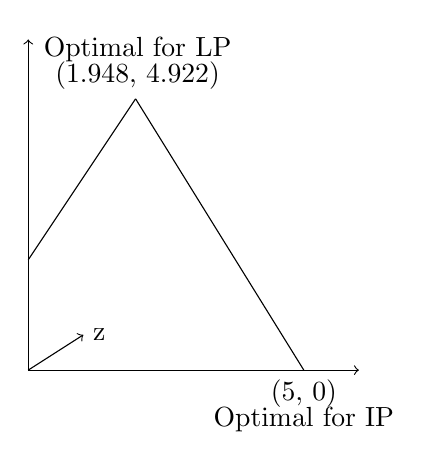
\begin{tikzpicture}[scale=0.7]
						\draw [->] (1,1) -- (1, 7);
						\draw [->] (1,1) -- (7, 1);
						\draw (1,3) -- (2.948, 5.922);
						\draw (2.948, 5.922) -- (6, 1);
						\draw [->] (1,1) -- (2, 1.64);
						\node [right] at (2, 1.64) {z};
						\node [above] at (2.984, 5.922) {(1.948, 4.922)};
						\node [above] at (2.984, 6.422) {Optimal for LP};
						\node [below] at (6,1) {(5, 0)};
						\node [below] at (6, 0.5) {Optimal for IP};
					\end{tikzpicture}
					\caption{Optimal solution for LP / IP}
				\end{figure}

			\subsection{Why Rounding Can be Bad - QAP example}
				Rounding can make the LP useless. For example, for QAP problem, the IP model is
				\begin{align}
					\text{min} \quad z &= \sum_{i\in D} \sum_{s\in O} c_is x_is + \sum_{i\in D} \sum_{j \in D} \sum_{s \in O} \sum_{t\in O} w_{ij}^{st}y_{ij}^{st}  \\
					\text{s.t.} \quad & \sum_{i \in D} x_{is} =1, \quad s\in D  \\
								&\sum_{s \in O} x_{is} = 1, \quad i \in D  \\
								&x_{is} \in \{0, 1\}, \quad i \in D, s\in O  \\
								& y_{ij}^{st} \ge x_{is} + x_{jt} - 1, \quad i\in D, j\in D, s\in O, t \in O  \\
								& y_{ij}^{st} \ge 0, \quad i\in D, j\in D, s\in O, t \in O  \\
								& y_{ij}^{st} \le x_{is}, \quad i\in D, j\in D, s\in O, t \in O  \\
								& y_{ij}^{st} \le x_{jt}, \quad i\in D, j\in D, s\in O, t \in O  
				\end{align}
				We can get the optimal solution for LP supposing $\forall i, s \quad x_{is}\in [0, 1]$
				\begin{align}
					x_{is} &= \frac{1}{|D|}, \quad i \in D, s\in O   \\
					y_{ij}^{st} & = 0, \quad i\in D, j\in D, s\in O, t \in O 
				\end{align}
				
			\subsection{IP and Convex Hull}
				For IP problem
				\begin{align}
					Z_{IP} \quad \text{max} \quad &z = cx  \\
							\text{s.t.} &Ax \le b \\
									&x\in {Z^n} 
				\end{align}
				In feasible region $S = \{x\in Z^n, Ax\le b\}$ , the optimal solution $Z_{IP} = \text{max}\{cx: x\in S\}$.\\
				Denote $conv(S)$ as the convex hull of $S$ then\\
				\begin{equation}Z_{IP}(S) = Z_{IP}(conv(S))  \end{equation}
				
			\subsection{Local Optimal and Global Optimal}
				Let 
				\begin{align}
					Z_s &= \text{min} \{f(x):x\in S\} \\
					Z_t &= \text{min} \{f(x):x\in T\}  \\
					& S \subset T 
				\end{align}
				then\\
				\begin{equation}Z_t \le Z_s  \end{equation}
				\textbf{Notice} that if $x_T^* \in S$ then $x_S^*=x_T^*$, to generalized it, \\
				We have
				\begin{align}
					\begin{cases}x_T^* \in \text{arg min} \{f(x): x\in T\} \\ x_T^* \in S\end{cases} \\ \Rightarrow x_T^*\in \text{arg min} \{f(x): x\in S\} 
				\end{align}
				Especially for IP, we can take the LP relaxation as $T$ and the original feasible region of IP as $S$, therefore, if we find an optimal solution from LP relaxation $T$ which is also a feasible solution of $S$, then it is the optimal solution for IP ($S$)
				
			\subsection{LP Relaxation}
				To perform the LP relaxation, we expand the feasible region
				\begin{align}
					x \in \{0,1\} & \rightarrow x\in [0, 1]  \\
					y\in Z^+ & \rightarrow y \ge 0 
				\end{align}
				If we have $Z_LP(s) = conv(s)$ then
				\begin{equation} LP(s): {x\in R_+^n: Ax\le b}\end{equation}
				The closer $LP(s)$ is to $conv(s)$ the better. Interestingly, we only need to know the convex in the direction of $c$.\\
				There are several formulation problem have the property of $Z_{LP}(s) = conv(s)$, such as:\\
				\indent- Assignment Problem\\
				\indent- Spawning Tree Problem\\
				\indent- Max Flow Problem\\
				\indent- Matching Problem

	\chapter{Decomposition Principle}

	\chapter{Ellipsoid Algorithm}

	\chapter{Projective Algorithm}

	\chapter{Interior-Point Algorithm}
	\part{Graph and Network Theory}
	\chapter{Paths, Trees, and Cycles}

	\chapter{Shortest-Path Problem}

	\chapter{Minimum Spanning Tree Problem}

	\chapter{Maximum Flow Problem}

	\chapter{Minimum Cost Flow Problem}

	\chapter{Assignment and Matching Problem}

	\chapter{Graph Algorithms}

	\chapter{Polygon Triangulation}
		\section{Types of Polygons}
			\framebox{\textbf{Def:}} A \textbf{simple polygon} is a closed polygonal curve without self-intersection.\\
			\begin{figure}[h!]
				\centering
				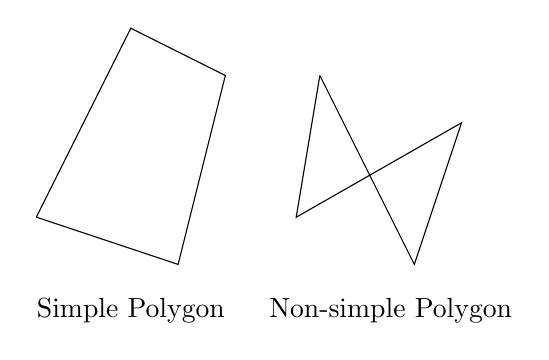
\begin{tikzpicture}[scale=0.6]
					\draw (0, 0) -- (3, -1) -- (4, 3) -- (2, 4) -- (0, 0);
					\draw (6, 3) -- (8, -1) -- (9, 2) -- (5.5, 0) -- (6, 3);
					\node at (2, -1.5) [below] {Simple Polygon};
					\node at (7.5, -1.5) [below] {Non-simple Polygon};
				\end{tikzpicture}
			\end{figure}\\
			Polygons are basic building blocks in most geometric applications. It can model arbitrarily complex shapes, and apply simple algorithms and algebraic representation/manipulation.
		\section{Triangulation}
			\framebox{\textbf{Def:}} \textbf{Triangulation} is to partition polygon $P$ into non-overlapping triangles using diagonals only. It reduces complex shapes to collection of simpler shapes. Every simple $n$-gon admits a triangulation which has $n-2$ triangles.\\
			\begin{figure}[h!]
				\centering
				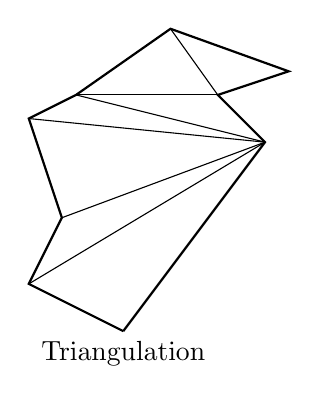
\begin{tikzpicture}[scale=0.6]
					\draw [thick] (0, 0) -- (3, 4) -- (2, 5) -- (3.5, 5.5) -- (1, 6.4) -- (-1, 5) -- (-2, 4.5) -- (-1.3, 2.4) -- (-2, 1) -- (0, 0);
					\draw (-2, 1) -- (3, 4);
					\draw (-1.3, 2.4) -- (3, 4);
					\draw (-2, 4.5) -- (3, 4);
					\draw (-1, 5) -- (3, 4);
					\draw (-1, 5) -- (2, 5);
					\draw (2, 5) -- (1, 6.4);
					\node at (0, 0) [below] {Triangulation};
				\end{tikzpicture}
			\end{figure}\\
			\framebox{\textbf{Theorem:}} Every polygon has a triangulation\\  
			\framebox{\textbf{Lemma:}} Every polygon with more than three vertices has a diagonal.\\
			\framebox{\textbf{Proof:}}(by Meisters, 1975) Let $P$ be a polygon with more than three vertices. Every vertex of a $P$ is either \textit{convex} or \textit{concave}. W.L.O.G.(any polygon must has convex vertex) Assume $p$ is a convex vertex. Denote the neighbors of $p$ as $q$ and $r$. If $\bar{qr}$ is a diagonal, done, and we call $\triangle{pqr}$ is an \textit{ear}. If $\triangle{pqr}$ is not an ear, it means at least one vertex is inside $\triangle{pqr}$, assume among those vertexes inside $\triangle{pqr}$, $s$ is a vertex closest to $p$, then $\bar{ps}$ is a diagonal. 
			
		\section{Art Gallery Theorem}
			\framebox{\textbf{Problem:}} The floor plan of an art gallery modeled as a simple polygon with $n$ vertices, there are guards which is stationed at fixed positions with 360 degree vision but cannot see through the walls. How many guards does the art gallery need for the security? (Fun fact: This problem was posted to Vasek Chvatal by Victor Klee in 1973)\\
			\framebox{\textbf{Theorem:}} Every $n$-gon can be guarded with $\lfloor \frac{n}{3} \rfloor$ vertex guards\\
			\framebox{\textbf{Lemma:}} Triangulation graph can be 3-colored.\\
			\framebox{\textbf{Proof:}} \\
			- $P$ plus triangulation is a planar graph\\
			- 3-coloring means there exist a 3-partition for vertices that no edge or diagonal has both endpoints within the same set of vertices.\\
			- Proof by Induction:\\
			\indent - Remove an ear (there will always exist ear) \\
			\indent - Inductively 3-color the rest\\
			\indent - Put ear back, coloring new vertex with the label not used by the boundary diagonal.

		\section{Triangulation Algorithms}



	\part{Integer and Combinatorial Programming}
	\chapter{Formulation}
		\section{Typical Problems}

		\section{Integer Programming Formulation Skills}
			\subsection{A Variable Taking Discontinuous Values}
				In algebraic notation: 
				\begin{equation}
					x = 0,\quad \text{or} \quad l\le x \le u 
				\end{equation}
				Modeling:
				\begin{align}
					& x \le uy \\
					& x \ge ly  \\
					& y \in \{0, 1\} 
				\end{align}
				where
				\begin{equation}y=\begin{cases}0, & \text{if }x=0 \\ 1, & \text{if } l\le x \le u\end{cases} \end{equation}
					
			\subsection{Fixed Costs}
				In algebraic notation: 
				\begin{equation}
					C(x) = \begin{cases} 0 & \text{for } x=0 \\ k + cx & \text{for } x > 0 \end{cases} 
				\end{equation}
				Modeling:
				\begin{align}
					& C^*(x, y) = ky+cx\\
					& x \le My  \\
					& x \ge 0 \\
					& y \in \{0, 1\} 
				\end{align}
				where
				\begin{equation}y=\begin{cases}0, & \text{if }x=0 \\ 1, & \text{if }x\ge 0\end{cases} \end{equation}
			
			\subsection{Either-or Constraints}
				In algebraic notation: 
				\begin{equation}
					\sum_{j\in J} a_{1j} x_j \le b_1 \text{ or } \sum_{j\in J} a_{2j} x_j \le b_2 
				\end{equation}
				Modeling:
				\begin{align}
					& \sum_{j\in J} a_{1j} x_j \le b_1 + M_1y  \\
					& \sum_{j\in J} a_{2j} x_j \le b_2 + M_1(1-y)  \\
					& y \in \{0, 1\} 
				\end{align}
				where
				\begin{equation}y=\begin{cases}0, & \text{if }\sum_{j\in J} a_{1j} x_j \le b_1 \\ 1, & \text{if } \sum_{j\in J} a_{2j} x_j \le b_2\end{cases} \end{equation}
				Notice that the sign before $M$ is determined by the inequality $\ge$ or $\le$, if it is \lq\lq{}$\ge$\rq\rq{}, use \lq\lq{}$-$\rq\rq{}, if it \lq\lq{}$\le$\rq\rq{}, use \lq\lq{}+\rq\rq{}.
			
			\subsection{Conditional Constraints}
				If constraint A is satisfied, then constraint B must also be satisfied
				\begin{equation}
					\text{If} \quad \sum_{j\in J} a_{1j} x_j \le b_1 \text{ then } \sum_{j\in J} a_{2j} x_j \le b_2 
				\end{equation}
				The key part is to find the opposite of the first condition. We are using $A\Rightarrow B \Leftrightarrow \neg B \Rightarrow \neg A$\\
				Therefore it is equivalent to
				\begin{equation}
					\sum_{j\in J} a_{1j} x_j > b_1 \text{ or } \sum_{j\in J} a_{2j} x_j \le b_2 
				\end{equation}
				Furthermore, it is equivalent to
				\begin{equation}
					\sum_{j\in J} a_{1j} x_j \ge b_1 + \epsilon \text{ or } \sum_{j\in J} a_{2j} x_j \le b_2 
				\end{equation}
				Where $\epsilon$ is a very small positive number.\\
				Modeling:
				\begin{align}
					& \sum_{j\in J} a_{1j} x_j \ge b_1 + \epsilon -  M_2y  \\
					& \sum_{j\in J} a_{2j} x_j \le b_2 + M_2(1-y)  \\
					& y \in \{0, 1\} 
				\end{align}	
			
			\subsection{Special Ordered Sets}
				Out of a set of yes-no decisions, at most one decision variable can be yes. Also known as SOS1.
				\begin{align}
					x_1=1,x_2=x_3&=\dots=x_n=0  \\
					&\text{or}  \\
					x_2=1, x_1=x_3&=\dots=x_n=0  \\
					&\text{or ...} 
				\end{align} 
				Modeling:
				\begin{equation} \sum_{i} x_i = 1, \quad i \in N \end{equation}
				Out of a set of binary variables, at most two variables can be nonzero. In addition, the two variables must be adjacent to each other in a fixed order list. Also known as SOS2.
				Modeling:
				If $x_1, x_2, ... , x_n$ is a SOS2, then
				\begin{align}
					& \sum_{i=1}^{n} x_i \le 2  \\
					& x_i + x_j \le 1, \forall i \in \{1, 2,..., n\}, j \in \{i+2, i+3, ..., n\}  \\
					&x_i \in \{0, 1\}
				\end{align}
				There is another type of definition, that is out of a set of nonnegative variables \textbf{not binary here}, at most two variables can be nonzero. In addition, the two variables must be adjacent to each other in a fixed order list. All variables summing to 1.\\
				This definition of SOS2 is used in Piecewise Linear Formulations.
								
			\subsection{Piecewise Linear Formulations}
				The objective function is a sequence of line segments, e.g. $y=f(x), $ consists $k-1$ linear segments going through $k$ given points $(x_1, y_1), (x_2, y_2), ... ,(x_k, y_k)$.\\
				Denote 
				\begin{equation}d_i=\begin{cases}1, & x\in (x_i, x_{i+1})\\0, & \text{otherwise} \end{cases}\end{equation}
				Then the objective function is
				\begin{equation}\sum_{i \in \{1, 2, ..., k-1\}} y = d_if_i(x) \end{equation} 
				Modeling: Given that objective function as a piecewise linear formulation, we can have these constraints\\
				\begin{align}
					&\sum_{i \in \{1, 2, ..., k-1\}} d_i =1  \\
					&d_i \in \{0, 1\}, i \in \{1, 2, ..., k-1\}  \\
					& x = \sum_{i \in \{1, 2, ..., k\}} w_i x_i  \\
					& y = \sum_{i \in \{1, 2, ..., k\}} w_i y_i  \\
					& w_1 \le d_1  \\
					& w_i \le d_{i-1} + d{i}, i \in \{2, 3, ..., k-1\}  \\
					& w_k \le d_{k-1} 
				\end{align}
				In this case, $ w_i \in SOS2$ (second definition)		
									
			\subsection{Conditional Binary Variables}
				Choose at most $n$ binary variable to be 1 out of  $x_1, x_2, ... x_m, m\ge n$. If $n=1$ then it is SOS1.\\
				Modeling:
				\begin{equation}
					\sum_{k\in \{1,2,...,m\}} x_k \le n
				\end{equation}
				Choose exactly $n$ binary variable to be 1 out of  $x_1, x_2, ... x_m, m\ge n$\\
				Modeling:
				\begin{equation}
					\sum_{k\in \{1,2,...,m\}} x_k = n
				\end{equation}
				Choose $x_j$ only if $x_k = 1$\\
				Modeling:
				\begin{equation}x_j = x_k  \end{equation}
				\lq\lq{}and\rq\rq{} condition, iff $x_1, x_2, ... , x_m =1$ then $y=1$\\
				Modeling:
				\begin{align}
					& y \le x_i, i\in \{1, 2, ..., m\}  \\
					& y \ge \sum_{i \in \{1, 2, ..., m\}} x_i - (m - 1) 
				\end{align}

			\subsection{Elimination of Products of Variables}
				For variables $x_1$ and $x_2$,
				\begin{equation}y = x_1 x_2\end{equation}
				Modeling: If $x_1, x_2$ are binary, it is the same as \lq\lq{}and\rq\rq{} condition of binary variables.\\
				If $x_1$ is binary, while $x_2$ is continuous and $0 \le x_2 \le u$, then
				\begin{align}
					y &\le ux_1  \\
					y &\le x_2  \\
					y &\ge x_2 - u(1- x_1)  \\
					y &\ge 0 
				\end{align}
				If both $x_1$ and $x_2$ are continuous, it is non-linear, we can use Piecewise linear formulation to simulate.

	\chapter{Polyhedral Analysis}
		\section{Polyhedral and Dimension}  
			\subsection{Polyhedral, Hyperplanes and Half-spaces}
				- A \textbf{polyhedron} is a set of the form $\{x\in \mathbb{R}^n|Ax\le b\}=\{x \in \mathbb{R}^n | a^ix\le b^i, \forall i \in M\}$, where $A \in \mathbb{R}^{m\times n}$ and $b \in \mathbb{R}^m$\\
				- A polyhedron $P \subset \mathbb{R}^n$ is \textbf{bounded} if there exists a constant $K$ such that $|x_i|<K, \forall x \in P, \forall i \in [1, n]$, in this case the polyhedron is call \textbf{polytopes}\\
				- The lower-bound of $K$ is called \textbf{diagonal} denoted by $d$\\
				
			\subsection{Open, Close Sets: boundary and interior}
				- Denote $N_\epsilon = \{y\in \mathbb{R}^n|\lVert y-x\rVert < \epsilon \}$ as the \textbf{neighborhood} of $x\in \mathbb{R}^n$\\						
				- Given $S\subseteq \mathbb{R}^n$, x belongs to the \textbf{interior} of $S$, denoted by $int(S)$ if there is $\epsilon > 0$ such that $N_\epsilon(x) \le S$\\
				- $S$ is said to be an \textbf{open set} iff $S=int(S)$\\
				- $x$ belongs to the \textbf{boundary} $\partial S$ if $\forall \epsilon >0$, $N_\epsilon(x)$ contains at least one point in $S$ and a point not in $S$\\
				- $x\in S$ belongs to the \textbf{closure} of $S$, denoted $cl(s)$ if $\forall \epsilon > 0$, $N_\epsilon(x) \cap S = \emptyset$
				- $S$ is called \textbf{closed} iff $S=cl(S)$\\
				- In IP, LP, MIP, etc. we always work with close set. No \lq\lq{}$<$\rq\rq{} or \lq\lq{}$>$\rq\rq{}
				
			\subsection{Hyperplane and half-space}
				- A \textbf{hyperplane} is $\{x\in \mathbb{R}^n|a^Tx=b\}$\\
				- A \textbf{half-space} is  $\{x\in \mathbb{R}^n|a^Tx\le b\}$
				
			\subsection{Dimension of Polyhedral}
				- A polyhedron $P$ is \textbf{dimension} $k$, denoted $dim(P)=k$, if the maximum number of affinely independent points in $P$ is $k+1$\\
				- A polyhedron $P\subseteq \mathbb{R}^n$ is \textbf{full-dimensional} if $dim(P) = n$\\
				- Let:\\
				\indent - $M=\{1, 2, ..., m\}$\\
				\indent - $M^= = \{i \in M | a_ix=b_i, \forall x \in P\}$, i.e. the equality set\\
				\indent - $M^\le = M \setminus  M^=$, i.e. the inequality set\\
				- Let $(A^=, b^=)$, $(A^\le, b^\le)$ be the corresponding rows of $(A, b)$\\
				- If $P\subseteq \mathbb{R}^n$, then $dim(P) = n - rank(A^=, b^=)$\\
				- To proof a constraint $(A^=, b^=)$ is an equality constraint, we need to proof all point in the closure of $P$ satisfied the constraint, to proof it is not an equality constraint, we need to find one point that is not in the hyperplane.
			
			\subsection{Dimension and Rank}
				- $x\in P$ is called an \textbf{inner point} of $P$ if $a^ix < b_i, \forall i \in M^\le$\\
				- $x\in P$ is called an \textbf{interior point} of $P$ if $a^ix<b_i, \forall i \in M$\\
				- Every nonempty polyhedron has at least one inner point\\
				- A polyhedron has an interior point iff $P$ is full-dimensional, i.e., there is no equality constraint
		
		\section{Face and Facet}
			\subsection{Valid Inequalities and Faces}
				- The inequality denoted by $(\pi, \pi_o)$ is called a \textbf{valid inequality} for $P$ if $\pi x \le \pi_0, \forall x \in P$\\
				- Note that $(\pi, \pi_0)$ is a valid inequality iff $P$ lies in the half-space $\{x\in \mathbb{R}^n|Ax\le b\}$\\
				\begin{figure}[!ht]
				\centering
				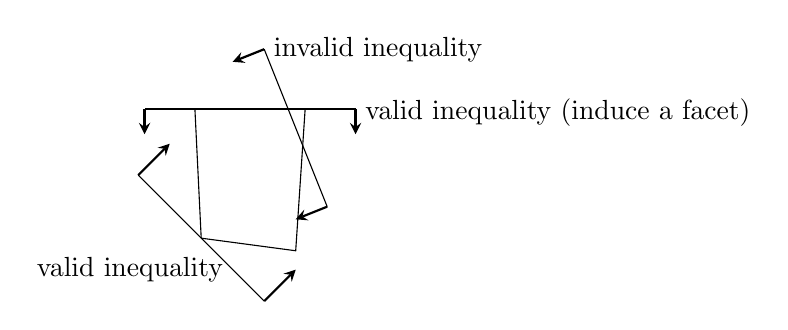
\begin{tikzpicture}[scale=0.4]
					\draw (0,0) -- (3, -0.4) -- (3.3, 4.1) -- (-0.2, 4.1) -- (0, 0);
					\draw (-2, 2) -- (2, -2);
					\draw (4.9, 4.1) -- (-1.8, 4.1);
					\draw (4, 1) -- (2, 6);
					\draw [arrow] (-1.8, 4.1) -> (-1.8, 3.3);
					\draw [arrow] (4.9, 4.1) -> (4.9, 3.3);
					\draw [arrow] (-2, 2) -> (-1, 3);
					\draw [arrow] (2, -2) -> (3, -1);
					\draw [arrow] (4, 1) -> (3, 0.6);
					\draw [arrow] (2, 6) -> (1, 5.6);
					\node at (1, -1) [left] {valid inequality};
					\node at (4.9, 4) [right] {valid inequality (induce a facet)};
					\node at (2, 6) [right] {invalid inequality};
				\end{tikzpicture}
				\caption{Example of valid/invalid inequality}
				\end{figure}
				- If $(\pi, \pi_0)$ is a valid inequality for $P$ and $F=\{x\in P|\pi x=x_0\}$, $F$ is called a \textbf{facet} of $P$ and we say that $(\pi, \pi_0)$ \textbf{represents} or \textbf{defines} $F$\\
				- A face is said to be \textbf{proper} if $F\ne \emptyset$ and $F\ne P$\\
				- The face represented by $(\pi, \pi_0)$ is nonempty iff $\max \{\pi x |x\in P\}=\pi_0\}$\\
				- If the face $F$ is nonempty, we say it \textbf{supports} $P$\\
				- Let $P$ be a polyhedron with equality set $M^=$. If 
				\begin{equation}F=\{x\in P | \pi^T x = \pi_0\}  \end{equation}
				is not empty, then $F$ is a polyhedron. Let 
				\begin{equation}M^= \subseteq M_F^=, M_F^{\le}=M \setminus M_F^= \end{equation}
				then 
				\begin{equation}F=\{x | a_i^T x=b_i, \forall i \in M_F^=, a_i^T x \le b_i, \forall i \in M_f^{\le}\} \end{equation}
				
			\subsection{Facet}
				- A face $F$ is said to be a \textbf{facet} of $P$ if $dim(F) = dim(P)-1$\\
				- Facets are all we need to describe polyhedral\\
				- If $F$ is a facet of $P$, then in any description of $P$, there exists some inequality representing $F$\\
				- Every inequality that represents a face that is not a facet is unnecessary in the description of $P$
				- Every full-dimensional polyhedron $P$ has a unique (up to scalar multiplication) representation that consists of one inequality representing each facet of $P$\\
				- If $dim(P) = n-k$ with $k>0$, then $P$ is described by a maximal set of linearly independent rows of $(A^=, b^=)$, as well as one inequality representing each facet of $P$
				
			\subsection{Proving Facet}
				To prove an inequality $\sum_i a_i x_i \le b_i$ is facet inducing for a $D$ dimensional polyhedral, we need to prove there are $D$ affinely independent vectors in $\sum_i a_i x_i = b_i$

			\subsection{Domination}
				$\Pi x\le \Pi_0$ dominates $Mx\le M_0$ if
				\begin{equation}
					\begin{cases}
						\Pi \ge \mu M, \mu > 0\\
						\Pi_0 \le \mu M_0, \mu > 0\\
						(\Pi, \Pi_0) \ne (M, M_0)
					\end{cases}
				\end{equation}

	\chapter{Branch and Bound}
		\section{LP based Branch and Bound}
			\subsection{Idea of Divide and Conquer}
				For each iteration, divide the feasible region of LP into two parts (and an infeasible part), solve the LP in those parts.\\
				\begin{figure}[!ht]
					\centering
					\begin{tikzpicture}[scale=0.5]
						\draw [<->] (10, 0) -- (0,0) -- (0,10);
						\draw (0, 8.5) -- (10, 2.5);
						\draw (2, 8) -- (9, 0);
						\draw [dashed] (3,0) -- (3,10);
						\draw [dashed] (4,0) -- (4,10);
						\node at (1.5, 5) {$S_1$};
						\node at (3.5, 4) {$S_2$};
						\node at (5, 3) {$S_3$}; 
					\end{tikzpicture}
					\caption{Divide and Conquer}
				\end{figure}
				In this iteration, the original feasible region have been partition into three parts, where $S_2$ is infeasible for IP because there is not integer point in it. We continue the iteration for $S_1$ and $S_2$. Each partition is suppose to give a new upper bound / lower bound and reduce the infeasible space.\\
				If the temp optimal integer in $S_1$ is larger than the LP relaxation in $S_3$, we can cut $S_3$.\\
				For each iteration, we use dual simple method, for the following two reasons:\\
				\indent - We can process new constraint very fast\\
				\indent - Always gives us a valid bound.\\
				
			\subsection{Relation Between LP Relaxation and IP}
				Let
				\begin{align}
					Z_{IP} &=\max_{x\in S} cx, \quad \text{where } s \text{ is a set of integer solutions} \\
					Z_{LP} &=\max cx, \quad \text{the LP relaxation of IP}  
				\end{align}
				then
				\begin{align}
					Z_{IP} &= \max_{1\le i \le k} \{\max_{x \in S_i} cx \} \\
					\text{iff} \quad S&=\bigcup_{1\le i \le k} S_i 
				\end{align}
				Notice that $S_i$ don\rq{}t need to be disjointed.\\
				\textbf{Important!} (For maximization problem)\\
				\indent - Any feasible solution provides a lower bound $L$, which is also the \textit{Prime Bound}\\
				\begin{equation}\hat{x}\in S \rightarrow Z_{IP}\ge c\hat{x}\end{equation}
				\indent - After branching, solving the LP relaxation over sub-feasible-region $S_i$ produces an upper bound, which is also the \textit{Dual Bound}, on each sub-problem\\
				\indent - If $u(S_i)\le L$, remove $S_i$\\
				\indent - LP can produce the first upper bound, but there might be possible to find other upper bound with other method (e.g. Lagrangian relaxation)
				
			\subsection{LP feasibility and IP(or MIP) feasibility}
				Solve the LP relaxation, one of the following things can happen\\
				\indent - LP is infeasible $\rightarrow$ MIP is infeasible\\
				\indent - LP is unbounded $\rightarrow$ MIP is infeasible or unbounded\\
				\indent - LP has optimal solution $\hat{x}$ and $\hat{x}$ are integer ($\hat{x} \in S$), $\rightarrow$ $Z_{IP} = Z_{LP}$\\
				\indent - LP has optimal solution $\hat{x}$ and $\hat{x}$ are not integer ($\hat{x} \notin S$), now defines a new upper bound, $Z_{LP} \ge Z_{IP}$\\
				If the first three happens, stop, if the fourth happens, we branch and recursively solve the sub-problems.
			
		\section{Terminology in Branch and Bound}
			- If we picture the sub-problems, they will form a \textbf{search tree} (typically a binary tree)\\
			- Each node in the search tree is a \textbf{sub-problem}\\
			- Eliminating a node is called \textbf{pruning}, we also stop considering its children\\
			- A sub-problem that has not being processed is called a \textbf{candidate}, we keep a list of candidates
			
		\section{Bounding}
		 	\textbf{Notice!} this section is for maximization, if it is for minimization, reverse upper bound and lower bound.
			\subsection{Upper Bound}
				- Upper bound it the Prime bound. which means it has to be a feasible solution\\
				- Some methods to get an upper bound:\\
				\indent - Rounding\\
				\indent - Heuristic\\
				\indent - Meta-heuristic
				
			\subsection{Lower Bound}
				- Lower Bound is the Dual bound,we can use LP relaxation to get it\\
				- The tighter the better, LP is better\\
				
		\section{Branch and Bound Algorithm}
			\begin{algorithm}[!ht]
				\caption{Branch and Bound}
				\begin{algorithmic}[1]
					\STATE find a feasible solution as the initial Lower bound $L$
					\STATE put the original LP relaxation in candidate list $S$
					\WHILE {$S \ne \emptyset$}
						\STATE select a problem $\hat{S}$ from $S$
						\STATE solve the LP relaxation of $\hat{S}$ to obtain $u(\hat{S})$
						\IF {LP is infeasible}
							\STATE $\hat{S}$ pruned by infeasibility
						\ELSIF {LP is unbounded}
							\STATE $\hat{S}$ pruned by unboundness or infeasibility
						\ELSIF{LP $u(\hat{S}) \le L$}
							\STATE $\hat{S}$ pruned by bound
						\ELSIF{LP $u(\hat{S}) > L$}
							\IF {$\hat{x}\in S$}
								\STATE $u(\hat{S})$ becomes new $L$, $L=u(\hat{S})$
							\ELSIF {$\hat{x}\notin S$}
								\STATE branch and add the new sub-problems to $S$
								\IF {LP $u(\hat{S})$ is at current best upper bound}
									\STATE set $U=u(\hat{S})$
								\ENDIF
							\ENDIF
						\ENDIF
					\ENDWHILE
					\IF {Lower bound exists}
						\STATE find the optimal at $L$
					\ELSE
						\STATE Infeasible
					\ENDIF
				\end{algorithmic}
			\end{algorithm}
	
		\section{The goal of Branching}
			- Divide the problem into easier sub-problems\\
			- We want to chose the branching variables that minimize the sum of the solution times of the sub-problems\\
			- If after branching the $u(S_i)$ changes a lot,\\
			\indent - I can find a good L first\\
			\indent - The branch may get worse than the current bound first\\
			- Instead of solving the potential two branches for all candidates to optimality, solve a few iterations of the dual simplex, each iteration of pivoting yields an upper bound.
			
		\section{Choose Branching Variables}
			\subsection{The Most Violated Integrality constraint}
				Pick the $j$ of which $x_j - \lfloor \hat{x_j} \rfloor$ is closer to 0.5
				
			\subsection{Strong Branching}
				Select a few candidates $(K)$, create all sub-problems for each of these variables, run a few dual simplex iterations to see the improved bounds, select the variable with the best bounds.\\
				for variable $x_j\in K$, we branch and do a few iterations to find two reductions of gaps, i.e. $D_j^+$ and $D_j^-$,
				\begin{figure}[!ht]
					\centering
					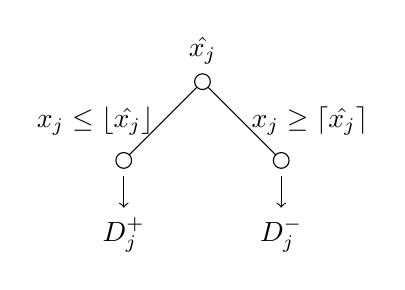
\begin{tikzpicture}[scale=0.2]
						\draw (0, 5) circle [radius=0.5];
						\draw (-5, 0) circle [radius=0.5];
						\draw (5, 0) circle [radius=0.5];
						\draw (0.353, 4.647) -- (4.647, 0.353);
						\draw (-0.353, 4.647) -- (-4.647, 0.353);
						\node [above] at (0, 5.5) {$\hat{x_j}$};
						\node [left] at (-2.5, 2.5) {$x_j \le \lfloor \hat{x_j} \rfloor$};
						\node [right] at (2.5, 2.5) {$x_j \ge \lceil \hat{x_j} \rceil$};
						\draw [->] (-5, -1) -- (-5, -3);
						\draw [->] (5, -1) -- (5, -3);
						\node [below] at (-5, -3) {$D_j^+$};
						\node [below] at (5, -3) {$D_j^-$};
					\end{tikzpicture}
					\caption{Strong Branching}
				\end{figure}
			
			\subsection{pseudo-cost Branching}
				Pseudo-cost is an estimate of per-unit change in the objective function, for each variable
				\begin{equation}\begin{cases}P_j^+, & \text{bound reduction if rounded up} \\ P_j^-, & \text{bound reduction if rounded down}\end{cases}\end{equation}
				define $f_j = x_j -\lfloor x_j \rfloor$
				\begin{equation}\begin{cases}D_j^+ = P_j^+ (1-f_j) \\ D_j^- = P_j^- f_j\end{cases}\end{equation}
		
		\section{Choose the Node to Branch}
			\subsection{Update After Branching}
				For those variables in $K$ find the \\
				- $\max \{\min\{ {D_j^+},  {D_j^-}\}\}$, or\\
				- $\max \{\max\{ {D_j^+},  {D_j^-}\}\}$, or\\
				- $\max \{\frac{D_j^+ + D_j^-}{2}\}$, or\\
				- $\max \{\alpha_1\min\{ {D_j^+},  {D_j^-}\} + \alpha_2\max\{ {D_j^+},  {D_j^-}\}\}$\\
				to branch.
		
			\subsection{Branch on Important Variables First}
				Branch on variables that affects many decisions.

			\subsection{Some Search Strategy}
				- Best Bound First: select the node with the largest bound (good for closing the gap)\\
				- Deep First: Good for finding Lower bound and easier to do dual simplex\\
				- Mix: Start with \lq\lq{}Deep First\rq\rq{} until we find a good bound and do \lq\lq{}Best Bound First\rq\rq{}

		\section{Types of Branching}
			\subsection{Traditional Branching}
				For $\hat{x} \notin S$, $\exists j \in N$ such that
				\begin{equation}\hat{x_j} -\lfloor\hat{x_j}\rfloor > 0 \end{equation}
				Create two sub-problems
				\begin{figure}[!ht]
					\centering
					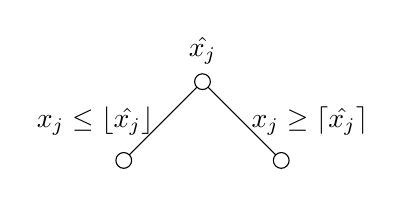
\begin{tikzpicture}[scale=0.2]
						\draw (0, 5) circle [radius=0.5];
						\draw (-5, 0) circle [radius=0.5];
						\draw (5, 0) circle [radius=0.5];
						\draw (0.353, 4.647) -- (4.647, 0.353);
						\draw (-0.353, 4.647) -- (-4.647, 0.353);
						\node [above] at (0, 5.5) {$\hat{x_j}$};
						\node [left] at (-2.5, 2.5) {$x_j \le \lfloor \hat{x_j} \rfloor$};
						\node [right] at (2.5, 2.5) {$x_j \ge \lceil \hat{x_j} \rceil$};
					\end{tikzpicture}
					\caption{Traditional Branching}
				\end{figure}

			\subsection{Constraint Branching}
				Use parallel constraints to branch, e.g.
				\begin{figure}[!ht]
					\centering
					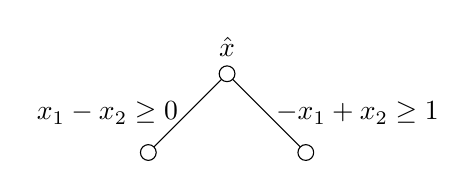
\begin{tikzpicture}[scale=0.2]
						\draw (0, 5) circle [radius=0.5];
						\draw (-5, 0) circle [radius=0.5];
						\draw (5, 0) circle [radius=0.5];
						\draw (0.353, 4.647) -- (4.647, 0.353);
						\draw (-0.353, 4.647) -- (-4.647, 0.353);
						\node [above] at (0, 5.5) {$\hat{x}$};
						\node [left] at (-2.5, 2.5) {$x_1 - x_2 \ge 0$};
						\node [right] at (2.5, 2.5) {$-x_1 + x_2 \ge 1$};
					\end{tikzpicture}
					\caption{Traditional Branching}
				\end{figure}
			
			\subsection{SOS}
				For SOS1,
				\begin{figure}[!ht]
					\centering
					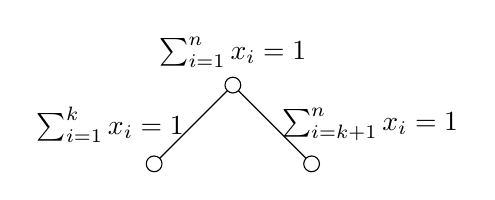
\begin{tikzpicture}[scale=0.2]
						\draw (0, 5) circle [radius=0.5];
						\draw (-5, 0) circle [radius=0.5];
						\draw (5, 0) circle [radius=0.5];
						\draw (0.353, 4.647) -- (4.647, 0.353);
						\draw (-0.353, 4.647) -- (-4.647, 0.353);
						\node [above] at (0, 5.5) {$\sum_{i=1}^{n}x_i=1$};
						\node [left] at (-2.5, 2.5) {$\sum_{i=1}^{k}x_i=1$};
						\node [right] at (2.5, 2.5) {$\sum_{i=k+1}^{n}x_i=1$};
					\end{tikzpicture}
					\caption{Traditional Branching}
				\end{figure}		
				For SOS2 (using the first definition),
				\begin{figure}[!ht]
					\centering
					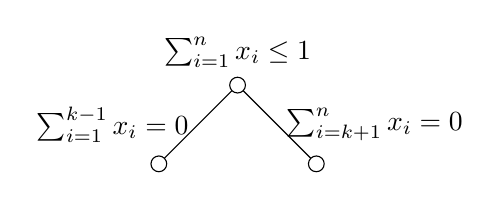
\begin{tikzpicture}[scale=0.2]
						\draw (0, 5) circle [radius=0.5];
						\draw (-5, 0) circle [radius=0.5];
						\draw (5, 0) circle [radius=0.5];
						\draw (0.353, 4.647) -- (4.647, 0.353);
						\draw (-0.353, 4.647) -- (-4.647, 0.353);
						\node [above] at (0, 5.5) {$\sum_{i=1}^{n}x_i \le 1$};
						\node [left] at (-2.5, 2.5) {$\sum_{i=1}^{k-1}x_i = 0$};
						\node [right] at (2.5, 2.5) {$\sum_{i=k+1}^{n}x_i =  0$};
					\end{tikzpicture}
					\caption{Traditional Branching}
				\end{figure}
			
			\subsection{GUB}
				This is where $x_i \in \{0, 1\}$, at most one variable can be 1,
				\begin{figure}[!ht]
					\centering
					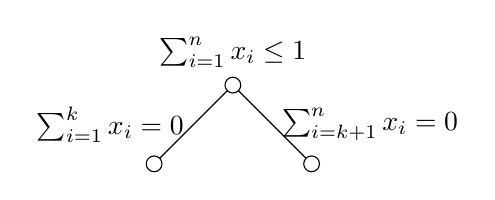
\begin{tikzpicture}[scale=0.2]
						\draw (0, 5) circle [radius=0.5];
						\draw (-5, 0) circle [radius=0.5];
						\draw (5, 0) circle [radius=0.5];
						\draw (0.353, 4.647) -- (4.647, 0.353);
						\draw (-0.353, 4.647) -- (-4.647, 0.353);
						\node [above] at (0, 5.5) {$\sum_{i=1}^{n}x_i\le 1$};
						\node [left] at (-2.5, 2.5) {$\sum_{i=1}^{k}x_i=0$};
						\node [right] at (2.5, 2.5) {$\sum_{i=k+1}^{n}x_i=0$};
					\end{tikzpicture}
					\caption{Traditional Branching}
				\end{figure}
			
			\subsection{Ryan-Foster}
				Ryan-Foster is for Set covering problem. The typical model is
				\begin{align}
					\text{min} \quad & \sum_{i \in C} x_i \\
					\text{s.t.} \quad & \sum_{i \in C} a_{ij}x_{i} \ge 1, \quad \forall j \in U \\
							& x_i \in \{0, 1\}, \quad \forall i \in C 
				\end{align}
				\textbf{Observation} For any fractional solution, there are at least two elements $(i,j)$ so that $i$ and $j$ are both partially covered by the same set $S$, but there is another set $T$ that only covers $i$
				\begin{figure}[!ht]
					\centering
					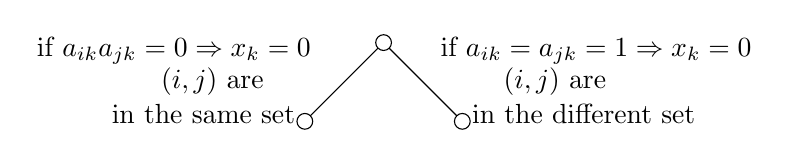
\begin{tikzpicture}[scale=0.2]
						\draw (0, 5) circle [radius=0.5];
						\draw (-5, 0) circle [radius=0.5];
						\draw (5, 0) circle [radius=0.5];
						\draw (0.353, 4.647) -- (4.647, 0.353);
						\draw (-0.353, 4.647) -- (-4.647, 0.353);
						\node [left] at (-7, 2.5) {$(i,j)$ are};
						\node [left] at (-5, 0.5) { in the same set};
						\node [left] at (-4, 4.5) {if $a_{ik}a_{jk}=0 \Rightarrow x_k = 0$};
						\node [right] at (7, 2.5) {$(i,j)$ are};
						\node [right] at (5, 0.5) { in the different set};
						\node [right] at (3, 4.5) {if $a_{ik}=a_{jk}=1 \Rightarrow x_k=0$};
					\end{tikzpicture}
					\caption{Traditional Branching}
				\end{figure}

	\chapter{Branch and Cut}
		\section{Separation Algorithm}
			Basic idea is to separate the feasible region so that the current "solution" (which is an fractional solution) is not included in the feasible region.
			\subsection{Vertices Packing}
				The current solution is $\bar{x} \in [0,1]^n$, we have two options to do the separation:\\
				\textbf{Option 1 - find the maximum clique:}\\
				(This approach is as hard as the original problem)\\
				denote
				\begin{equation}
					y_i=\begin{cases}1, \text{ if } i \in C \\ 0, \text{ otherwise}\end{cases}
				\end{equation}
				Find the maximum clique via:
				\begin{align}
					\max \quad &\sum \bar{x_i} y_i  \\
					\text{s.t.} \quad & y_i + y_j \le 1, \forall \{i, j\} \notin E 
				\end{align}
				\textbf{Option 2 - Heuristic:}
				\begin{algorithm}[!ht]
					\caption{Heuristic method to find a clique}
					\begin{algorithmic}[1]
						\STATE find $v=\text{argmax}_{i\in V} \{\bar{x_i}\}, C=\{v\}$
						\WHILE {$u\in \text{argmax}_{i \in \cap_{i \notin C}N_{(i, j)}\notin C} \{\bar {x_1}\}$ exists}
							\STATE C.add(u)
						\ENDWHILE
						\STATE return C
					\end{algorithmic}
				\end{algorithm}\\
				If $\sum_{i\in C} \bar{x_i} > 1$ then add cut $\sum_{i\in C} x_i \le 1$

			\subsection{TSP}
				When we have a solution, i.e. $\bar{x}$, perform the sub-tour searching algorithm, if there exists any sub-tour, add the corresponded constraint. That is the separation.

		\section{Optional v.s. Essential Inequalities}
			\subsection{Valid (Optional) Inequalities}
				See Figure \ref{OptInq}
				\begin{figure}[!ht]
					\centering
					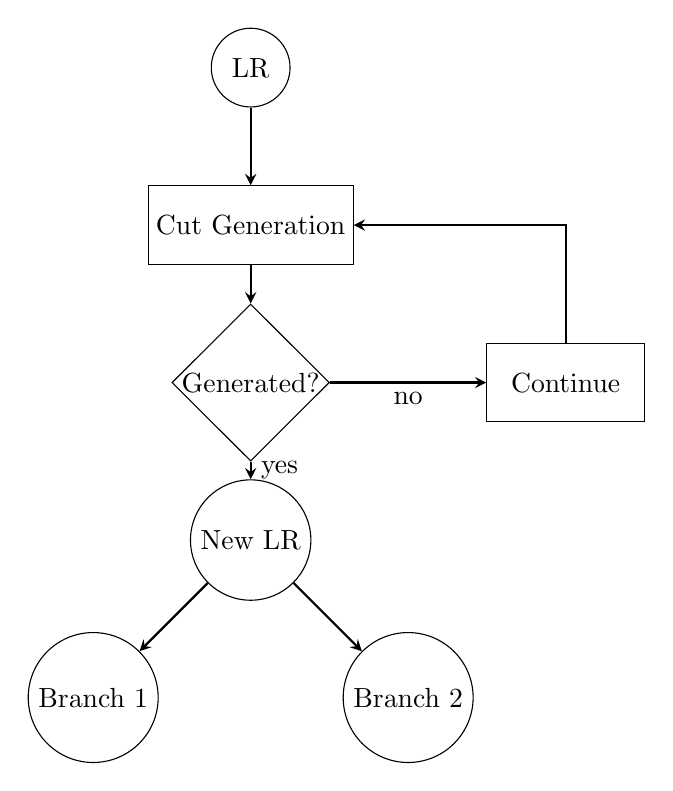
\begin{tikzpicture}[node distance = 2cm]
						\node (LR) [circleNode] {LR};
						\node (CG) [process, below of=LR] {Cut Generation};
						\node (CLimit) [decision, below of=CG] {Generated?};
						\node (Cont) [process, below of=CG, xshift=4cm] {Continue};
						\node (NLR) [circleNode, below of=CLimit] {New LR};
						\node (LNLR) [circleNode, below of=NLR, xshift=-2cm] {Branch 1};
						\node (RNLR) [circleNode, below of=NLR, xshift=2cm] {Branch 2};
						\draw [arrow] (LR) -- (CG);
						\draw [arrow] (CG) -- (CLimit);
						\draw [arrow] (CLimit) -- node [right] {yes} (NLR);
						\draw [arrow] (CLimit) -- node [below] {no} (Cont);
						\draw [arrow] (Cont) |- (CG);
						\draw [arrow] (NLR) -- (LNLR);
						\draw [arrow] (NLR) -- (RNLR);
					\end{tikzpicture}
					\caption {Branch and Cut for Optional Inequality}\label{OptInq}
				\end{figure}

			\subsection{Essential Inequalities (Lazy Cuts)}
				See Figure \ref{EssInq}
				\begin{figure}[!ht]
					\centering
					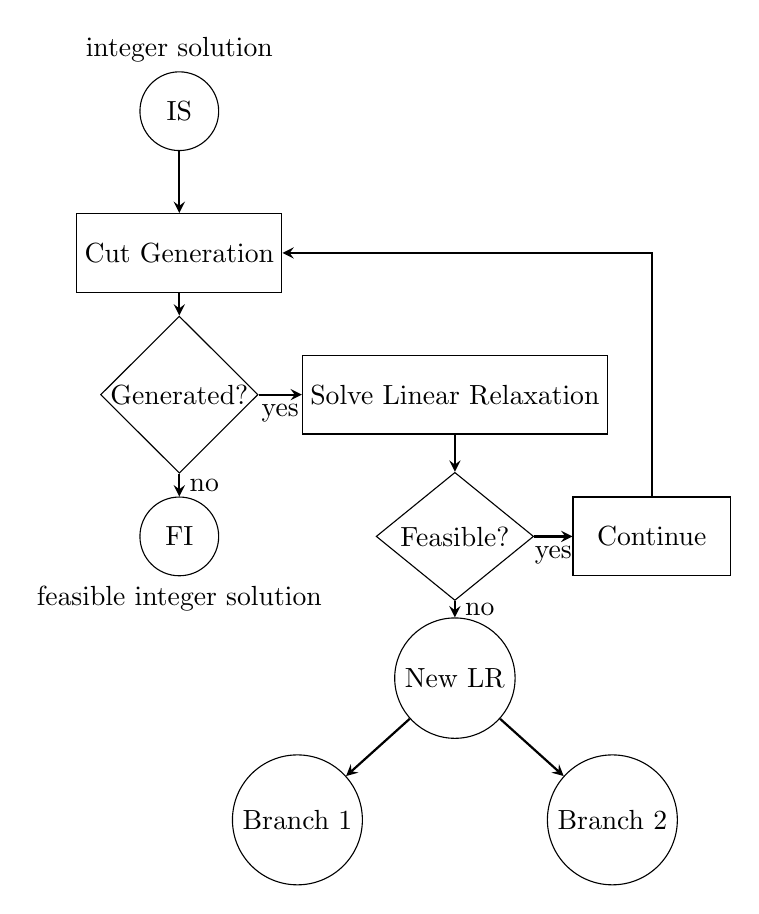
\begin{tikzpicture}[node distance = 1.8cm]
						\node (IS) [circleNode, label = above:integer solution] {IS};
						\node (CG) [process, below of=IS] {Cut Generation};
						\node (CLimit) [decision, below of=CG] {Generated?};
						\node (FI) [circleNode, below of=CLimit, label = below:feasible integer solution] {FI};
						\node (LP) [process, below of=CG, xshift = 3.5cm] {Solve Linear Relaxation};
						\node (LPF) [decision, below of=LP] {Feasible?};
						\node (NLR) [circleNode, below of=LPF] {New LR};
						\node (LNLR) [circleNode, below of=NLR, xshift=-2cm] {Branch 1};
						\node (RNLR) [circleNode, below of=NLR, xshift=2cm] {Branch 2};
						\node (Cont) [process, below of=LP, xshift=2.5cm] {Continue};
						\draw [arrow] (IS) -- (CG);
						\draw [arrow] (CG) -- (CLimit);
						\draw [arrow] (CLimit) -- node [right] {no} (FI);
						\draw [arrow] (CLimit) -- node [below] {yes} (LP);
						\draw [arrow] (LP) -- (LPF);
						\draw [arrow] (LPF) -- node [right] {no} (NLR);
						\draw [arrow] (LPF) -- node [below] {yes} (Cont);
						\draw [arrow] (NLR) -- (LNLR);
						\draw [arrow] (NLR) -- (RNLR);
						\draw [arrow] (Cont) |- (CG);
					\end{tikzpicture}
					\caption {Branch and Cut for Essential Inequality}\label{EssInq}
				\end{figure}

		\section{Chvatal-Gomory Cut}
			\subsection{Chvatal-Gomory Rounding Procedure}
				For $x=P\cap \mathbb{Z}_+^n$, where $P=\{x\in \mathbb{R}_+^n|Ax \le b\}$, A is an mxn matrix with columns $\{a_1, ..., a_n\}$ and $u \in \mathbb{R}_+^n$\\
				- The inequality
				\begin{equation}
					\sum_{j=1}^n ua_jx_j\le ub 
				\end{equation}
				is valid\\
				- Therefore the inequality
				\begin{equation}
					\sum_{j=1}^n \lfloor ua_j \rfloor x_j \le ub 
				\end{equation}
				is valid\\
				- Furthermore, the inequality
				\begin{equation}
					\sum_{j=1}^n \lfloor ua_j \rfloor x_j \le \lfloor ub \rfloor 
				\end{equation}
				is valid.

			\subsection{Gomory Cutting Plane}
				For a IP problem
				\begin{align}
					\max \quad & cx  \\
					\text{s.t.} \quad & Ax=b  \\
						& x \in \mathbb{B}^n 
				\end{align}
				let $\bar{x}$ be an optimal basic solution for the LR of P.
				\begin{equation}
					\bar{x} = \left[\begin{matrix} B^{-1}b \\ 0 \end{matrix}\right] = \left[ \begin{matrix}x_B \\ x_N\end{matrix}\right] 
				\end{equation}
				We have
				\begin{align}
					& Bx_B + Nx_N = b \\
					\Rightarrow \quad & x_B + B^{-1}Nx_N=B^{-1}b  \\
					\Rightarrow \quad & x_B + [\bar{a}_1, \bar{a}_2, ...]x_N = \bar{b} \\
					\Rightarrow \quad & x_i + \sum_{j\in NB} \bar{a}_{ij}x_j = \bar{b}_i \quad \text{(for the $i$th row)} 
				\end{align}
				Assume that $x_i \in \{0, 1\}$, use CG-Procedure
				\begin{equation}
					x_i + \sum_{j \in NB} \lfloor \bar{a}_{ij} \rfloor x_j \le \lfloor \bar{b}_i \rfloor 
				\end{equation}
				is a valid constraint for $P$, furthermore,
				\begin{equation}
					(\bar{b}_i - \sum_{j\in NB} \bar{a}_{ij}x_j) + \sum_{j\in NB}\lfloor \bar{a}_{ij} \rfloor x_j\le \lfloor \bar{b}_i \rfloor 
				\end{equation}
				Move the item, we get a new Gomory Cutting Plane
				\begin{equation}
					\sum_{j\in NB} (\bar{a}_{ij} - \lfloor \bar{a}_{ij} \rfloor)x_j \ge \bar{b}_i - \lfloor \bar{b}_i \rfloor  
				\end{equation}
				Add this inequality to the LR, use the dual simplex method to do one pivot, we get a new solution. Use Gomory cutting plane iteratively and we can find the optimal solution for IP.

	\chapter{Typical IP problems}
		\section{Packing and Matching}
			\subsection{Vertices Packing Formulation}
				Given a graph $G=(V, E)$, with $|V|=n$. A vertices packing solution is that no two neighboring vertices can be chosen at the same time.
				\begin{equation}
					PACK(G) = \{x\in \mathbb{B}^n|x_i + x_j \le 1, \forall (i, j)\in E\} 
				\end{equation}
				\framebox{\textbf{Example:}}
				\begin{figure}[!ht]
					\centering
					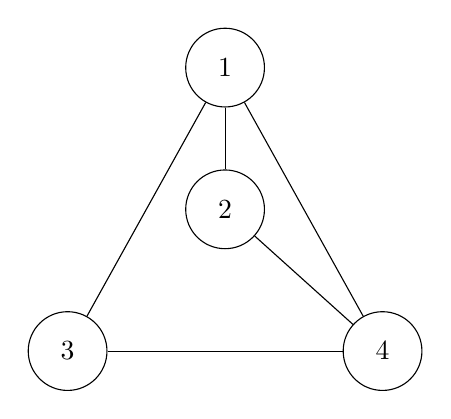
\begin{tikzpicture}[node distance = 1.8cm]
						\node (1) [circleNode] {1};
						\node (2) [circleNode, below of=1] {2};
						\node (3) [circleNode, below of=2, xshift=-2cm] {3};
						\node (4) [circleNode, below of=2, xshift=2cm] {4};
						\draw (1) -- (2);
						\draw (1) -- (3);
						\draw (1) -- (4);
						\draw (2) -- (4);
						\draw (3) -- (4);
					\end{tikzpicture}
					\caption{Example of vertices packing problem}
				\end{figure}
				The PACK of this graph is\\
				\begin{equation}
					PACK = conv\left(
						\left(\begin{matrix}0 \\ 0 \\ 0 \\ 0\end{matrix}\right),
						\left(\begin{matrix}1 \\ 0 \\ 0 \\ 0\end{matrix}\right),
						\left(\begin{matrix}0 \\ 1 \\ 0 \\ 0\end{matrix}\right),
						\left(\begin{matrix}0 \\ 0 \\ 1 \\ 0\end{matrix}\right),
						\left(\begin{matrix}0 \\ 0 \\ 0 \\ 1\end{matrix}\right),
						\left(\begin{matrix}0 \\ 1 \\ 1 \\ 0\end{matrix}\right)
						\right)
				\end{equation}

			\subsection{Matching Formulation}
				Given a graph $G=(V, E)$, denote $\delta(i)$ as the set of all the edges introduced to vertice $i\in V$. A matching solution is that no two edges introduced to the same vertice can be chosen at the same time.
				\begin{equation}
					MATCH(G) = \{\sum_{e\in \delta(i)}x_e \le 1|i\in V\}
				\end{equation}

			\subsection{Dimension of PACK(G)}
				The dimension of PACK, i.e. $dim(PACK(G))$ is (full-dimensional)
				\begin{equation}
					dim(PACK(G)) = |V| 
				\end{equation}
				To prove that $dim(PACK(G)) = |V|$, we need to find $|V| + 1$ affinely independent vectors.\\
				\framebox{\textbf{Proof:}}\\
					\begin{equation}
						rank\left(\left[\begin{matrix}0 & I_{|V|} \\ 1 & 1\end{matrix}\right]\right) = |V| + 1 
					\end{equation}
				Therefore, in PACK, $rank(A^=,b^=)=0$ 
			
			\subsection{Clique}
				- A \textbf{clique} is a subset of a graph that in the clique every two vertices linked with each other (complete sub-graph).
				- A \textbf{maximum clique} is a clique that any other vertice can not form a clique with all the points in this clique.

			\subsection{Inequalities and Facets of conv(VP)}
				\framebox{\textbf{Example:}}\\
					\begin{figure}[!ht]
						\centering
						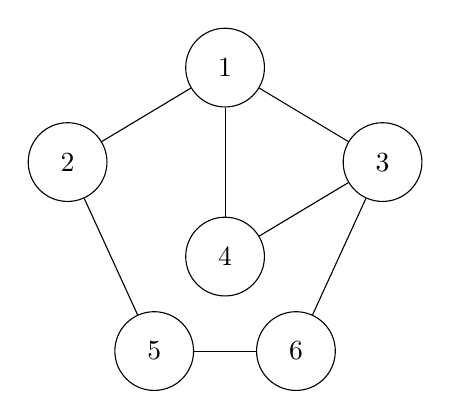
\begin{tikzpicture}[node distance = 1.2cm]
							\node (1) [circleNode] {1};
							\node (2) [circleNode, below of=1, xshift=-2cm] {2};
							\node (3) [circleNode, below of=1, xshift=2cm] {3};
							\node (4) [circleNode, below of=2, xshift=2cm] {4};
							\node (5) [circleNode, below of=4, xshift=-0.9cm] {5};
							\node (6) [circleNode, below of=4, xshift=0.9cm] {6};
							\draw (1) -- (2);
							\draw (1) -- (3);
							\draw (1) -- (4);
							\draw (3) -- (4);
							\draw (2) -- (5);
							\draw (5) -- (6);
							\draw (6) -- (3);
						\end{tikzpicture}
						\caption{Example}
					\end{figure}

				\subsubsection{Type 1 (Nonnegative Constraints)}
					$x_i \ge 0$ induce facets.\\
					\framebox{\textbf{Proof:}}
					\begin{equation}
						rank\left(\left[\begin{matrix}0 & 0 \\ 0 & I_{|V|}\end{matrix}\right]\right) = |V| + 1 
					\end{equation}

				\subsubsection{Type 2 (Neighborhood Constraints)}
					$x_i + x_j \le 1$ is a valid constraint, but it \textbf{DOES NOT} always induce facet.

				\subsubsection{Type 3 (Odd Hole)}
					$H$ is an odd hole if it contains circle of $k$ nodes, such that $k$ is odd and there is no cords. e.g. \{1, 2, 5, 6, 3\}. Then, the following inequality is valid,
					\begin{equation}
						\sum_{i\in H}x_i\le \frac{|H|-1}2 
					\end{equation}
					Odd Hole inequality \textbf{DOES NOT} always induce facets.\\
					This inequality can be derived from Gomory cut.

				\subsubsection{Type 4 (Maximum Clique)}
					$C$ is a maximum clique, then the following inequality is valid and induce a facet,
					\begin{equation}
						\sum_{i\in C} x_i \le 1 
					\end{equation}
					\framebox{\textbf{Proof:}}\\
						First, if $C=V$
						\begin{equation}
							rank\left(\left[I\right]\right) = |C| = |V| 			
						\end{equation}
						Second, if $C$ is a subset of $V$, for each vertice in $V \setminus C$, there should be at least one vertice in $C$ that is not linked with it. Therefore for each vertice in $C$ we can find a packing.

			\subsection{Gomory Cut in Set Covering}
				Consider a graph $G=(V, E)$, the covering problem is
				\begin{equation}
					\sum_{e\in \delta(i)}x_e \le 1, i\in V, x_e\in \{0, 1\}, e\in E
				\end{equation}
				For $T\subset V$, denote $\delta(i)$ as all edges induce to $i\in V$, denote $E(T) \subset E$ as all the edges linked between $(i, j), i\in T, j\in T$, therefore we have
				\begin{equation}
					\sum_{i\in T}\sum_{e\in \delta(i)}x_e \le |T| 
				\end{equation}
				For edges linking $i \in T, j \in T$, count them twice, for edges linking $i\in T, j\notin T$, count them once.We can have a new constraint
				\begin{equation}
					2\sum_{e\in E(T)}x_e + \sum_{e\in \delta(V\setminus T, T)}x_e \le |T| 
				\end{equation}
				Perform the Gomory Cut, the following constraint is a valid:
				\begin{equation}
					\sum_{e\in E(T)}x_e \le \lfloor \frac{|T|}2 \rfloor 
				\end{equation}
							
		\section{Traveling Salesman Problem}
			\subsection{TSP Formulation (Asymmetric)}
				Consider a Graph $G=\{A, N\}$\\
				Denote:\\
				\begin{equation}
					x_{ij} = \begin{cases}1, &\text{if goes from } i \text{ to } j\\ 0, & \text{otherwise}\end{cases}
				\end{equation}
				\textbf{Dantzig-Fulkerson-Johnson Formulation:}
				\begin{align}
					\min &\sum_{(i, j)\in A} c_{ij}x_{ij} \\
					& \sum_{j \in N, (i,j)\in A} x_{ij} = 1 \\
					& \sum_{i \in N, (i,j)\in A} x_{ij} = 1 \\
					& \sum_{j\notin S, i\in S, (i,j)\in A} x_{ij} = 1\text{ or } \sum_{i, j \in S, (i, j) \in A} x_{ij} \le |S| - 1 \\
					& \forall S \subset N, S\ne \emptyset, 2\le |S| \le n-1 
				\end{align}
				\textbf{Miller-Tucker-Zemlin Formulation:}
				\begin{align}
					\min &\sum_{(i, j)\in A} c_{ij}x_{ij} \\
					& \sum_{j \in N, (i,j)\in A} x_ij = 1 \\
					& \sum_{i \in N, (i,j)\in A} x_ij = 1 \\
					& u_i - u_j +nx_{ij}\le n-1 \quad i, j\in{2, ... , n}, (i, j)\in A \\
					& u_1 = 1 \\
					& 2 \le u_i \le n, i\in N, i>1 
				\end{align}

			\subsection{Sub-tour Searching Algorithm}
				In the graph $G=(N, A)$, let $\bar{G}=(N, \bar{A})$ be the connected components of graph, where
				\begin{equation}\bar{G}=(G, \bar{A}), \bar{A}=\{(i, j) \in A | \bar{x_{ij}}=1\} \end{equation}
				denote
				\begin{equation}\bar{FS}(i) = \{(i,j)\in \bar{A}\} \end{equation}
				Then the algorithm to find all sub-tour is the following:
				\begin{algorithm}[!ht]
					\caption{Sub-tour Searching Algorithm}
					\begin{algorithmic}[1]
						\STATE $K = \emptyset$
						\STATE $d_i = 0, \forall i \in N$
						\FOR {$i\in N$}
							\STATE $C = \emptyset$
							\STATE $Q = \emptyset$
							\IF {$d_i == 0$}
								\STATE $d_i = 1$
								\STATE $C = C\cup \{i\}$
								\STATE Q.append(i)
								\WHILE {$Q\ne \emptyset$}
									\STATE v = Q.pop()
									\FOR {$u \in \bar{FS}(v)$}
										\IF {$d_u == 0$}
											\STATE $d_u = 1$
											\STATE $C = C \cup \{u\}$
											\STATE Q.append(u)
										\ENDIF
									\ENDFOR
								\ENDWHILE
							\ENDIF
							\STATE $K=K\cup C$
						\ENDFOR
					\end{algorithmic}
				\end{algorithm}
			
		\section{Knapsack Problem}
			\subsection{Knapsack Problem Formulation}
				Consider the knapsack set KNAP
				\begin{equation}conv(KNAP)= conv(\{x\in \mathbb{B}^n|\sum_{j\in N}a_jx_j\le b\})\end{equation}
				in where\\
				- $N = \{1, 2, ..., n\}$\\
				- With out lost of generality, assume that $a_j > 0, \forall j \in N$ and $a_j < b, \forall j \in N$

			\subsection{Valid Inequalities for a Relaxation}
				For $P=\{x\in \mathbb{B}^n | Ax\le b\}$, each row can be regard as a Knapsack problem, i.e. for row $i$
				\begin{equation}
					P_i = \{x\in \mathbb{B}^n | a_i^T x \le b_i\} 
				\end{equation}
				is a relaxation of $P$, therefore,
				\begin{equation}
					P\subseteq P_i, \forall i=1,2,...,m 
				\end{equation}
				\begin{equation}
					P\subseteq \cap_{i=1}^m P_i 
				\end{equation}
				So any inequality valid for a relaxation of an IP is also valid for IP itself.
				
			\subsection{Cover and Extended Cover}
				A set $C\subseteq N$ is a cover if $\sum_{j\in C} a_j > b$, a cover $C$ is minimal cover if
				\begin{equation}
					C\subseteq N | \sum_{j\in C}a_j>b, \sum_{j\in C\setminus k} a_j < b, \forall k \in C 
				\end{equation}
				For a cover $C$, we can have the cover inequality
				\begin{equation}
					\sum_{j\in C}x_j \le |C|-1
				\end{equation}
				The inequality is trivial considering the pigeonhole principle.\\
				$C\subseteq N$ is a minimal cover, then $E(C)$ is defined as following:
				\begin{equation}
					E(C) = C\cup \{j \in N | a_j \ge a_i, \forall i \in C\}
				\end{equation}
				is called an extended cover. Then we have,
				\begin{equation}
					\sum_{i\in E(C)} x_i \le |C| - 1 \text{ dominates } \sum_{i\in C} x_i \le |C| - 1
				\end{equation}
				and
				\begin{equation}
					\sum_{i\in E(C)} x_i \le |C| - 1 \text{ dominates } \sum_{i\in E(C)} x_i \le |E(C)| - 1
				\end{equation}
				Hereby we need to prove that $\sum_{i\in E(C)} x_i \le |C| - 1$ is valid, by contradiction.\\
				\framebox{\textbf{Proof:???}} Suppose $x^R \in KNAP$, $R$ is a feasible solution, Where
				\begin{equation}
					x^R_j = \begin{cases}1, \quad \text{if $j\in R$} \\ 0, \quad \text{otherwise}\end{cases} 
				\end{equation}
				Then
				\begin{equation}
					\sum_{j\in E(C)}x^R_j \ge |C| \Rightarrow |R \cap E(C)| \ge |C|  
				\end{equation}
				therefore
				\begin{equation}
					\sum_{j\in R}a_j \ge \sum_{j\in R \cap E(C)} a_j \ge \sum_{j\in C} a_j > b 
				\end{equation}
				which means $R$ is a cover, it is contradict to $\sum_{j\in E(C)}x^R_j \ge |C|$ so $x^R \notin KNAP$

			\subsection{Dimension of KNAP}
				$conv(KNAP)$ is full dimension, i.e. $dim(conv(KNAP))=n$.\\
				\framebox{\textbf{Proof:}} $0, e_j, \forall j\in N$ are $n + 1$ affinely independent points in $conv(KNAP)$\\

			\subsection{Inequalities and Facets of conv(KNAP)}
				\subsubsection{Type 1 (Lower Bound and Upper Bound Constraints):}
					- $x_k\ge 0$ is a facet of $conv(KNAP)$\\
					\framebox{\textbf{Proof:}} $0, e_j, \forall j\in N\setminus k$ are $n$ affinely independent points that satisfied $x_k=0$\\
					- $x_k\le 1$ is a facet iff $a_j + a_k \le b, \forall j\in N \setminus k$\\
					\framebox{\textbf{Proof:}} $e_k, e_j+e_k, \forall j \in N\setminus k$ are $n$ affinely independent points that satisfied $x_k = 1$

				\subsubsection{Type 2 (Extended Cover)}
					Order the variables so that $a_1 \ge a_2 \ge \dots \ge a_n$, therefore $a_1 = a_{max}$\\
					Let $C$ be a cover with $\{j_1, j_2, \dots, j_r\}$ where $j_1 < j_2 < \dots < j_r$ so that $a_{j_1} \ge a_{j_2} \ge \dots \ge a_{j_r}$\\
					Let $p = \min\{j | j\in N \setminus E(C)\}$\\
					Then
					\begin{equation}
						\sum_{j\in E(C)} x_j \le |C| - 1 
					\end{equation}
					is a facet of $conv(KNAP)$ if\\
					- $C = N$\\
					\framebox{\textbf{Proof:}}
					\begin{equation}
						R_k = C\setminus k, \forall k \in C = N \setminus k, \forall k \in N 
					\end{equation}
					have $|N|$ affinely independent vectors\\
					- $E(C) = N$ and $\sum_{j\in C \setminus \{j_1, j_2\}} a_j + a_{max} \le b$\\
					\framebox{\textbf{Proof:}} ($j_1, j_2$ are two heaviest elements in $C$)
					\begin{equation}
						S_k = C\setminus \{j_1, j_2\}\cup \{k\}, \forall k\in E(C)\setminus C 
					\end{equation}
					$R_k\cup S_k$ have $|C|+|E(C) \setminus C| = |E(C)| = |N|$ affinely independent vectors\\
					- $C = E(C)$ and $\sum_{j\in C \setminus j_1} a_j + a_p \le b$)\\
					\framebox{\textbf{Proof:}} ($j_1$ is the heaviest element in $C$, $k$ is the lightest element outside extended cover)
					\begin{equation}
						T_k = C \setminus j_i \cup \{k\}, \forall k\in N\setminus E(C) 
					\end{equation}
					$R_k \cup T_k$ have $|N \setminus E(C)| + |E(C)| = |N\setminus C| + |C| = |N|$ affinely independent vectors\\
					- $C \subset E(C) \subset N$ and $\sum_{j\in C \setminus \{j_1, j_2\}} a_j + a_{max} \le b$ and $\sum_{j\in C \setminus j_1} a_j + a_p \le b$\\
					\framebox{\textbf{Proof:}}$S_k \cup T_k$ have $|E(C) \setminus C| + |N \setminus E(C)| = |N|$ affinely independent vectors

			\subsection{Lifting}
				\subsubsection{Up Lifting}
					For KNAP problem
					\begin{equation}
						KNAP = \{x\in \mathbb{B}^n | \sum_j a_jx_j \le b\} 
					\end{equation}
					For $P=conv(KNAP)$ denote\\
					\begin{align}
						&P_{k_1, k_2, ..., k_m} \\
						&\quad =conv(KNAP\cap \{x\in \mathbb{B}^{n}|x_{k_1}=x_{k_2}=\dots=x_{k_m}=0\}) 
					\end{align}
					Therefore
					\begin{align}
						&P_{k_1, k_2, ..., k_m} \\
						&\quad=conv(KNAP\cap \{x\in \mathbb{B}^{n}|\sum_{j\in N\setminus \{k_1, k_2, ..., k_m\}} a_j x_j \le b\}) 
					\end{align}
					The $C=N$ cover inequality for $P_{k_1, k_2, ..., k_m}$ implies
					\begin{equation}
						\sum_{j\in N\setminus \{k_1, k_2, ..., k_m\}} x_j \le n-m-1 
					\end{equation}
					is a facet of $P_{k_1, k_2, ..., k_m}$\\
					The lifting process is to find a facet for $P_{k_1, k_2, ..., k_{m-1}}$ using facet of $P_{k_1, k_2, ..., k_m}$, i.e. find $\alpha_{m}$ for the following constraint to be a facet.
					\begin{equation}
						\alpha_m x_m + \sum_{j\in N\setminus \{k_1, k_2, ..., k_m\}} x_j \le n-m-1 
					\end{equation}
					If $x_m=0$, $\alpha_m \ge 0$,\\
					If $x_m=1$, $\alpha_m \le (n-m+1) - \gamma$ where
					\begin{align}
						\gamma &= \max\{\sum_{j\in N\setminus\{k_1, k_2, ..., k_m\}}x_j|x\in P_{k_1, k_2, ..., k_{m-1}}, x_m=1\} \\
						&= \max\{\sum_{j\in N\setminus\{k_1, k_2, ..., k_m\}}x_j|\sum_{j \in N \setminus \{k_1, k_2, ..., k_m\}}a_jx_j\le b-a_m\} 
					\end{align}
					Then let $\alpha_m = n-m+1-\gamma$, we uplifted a constraint. Repeat this procedure for $\{k_1, k_2, ..., k_m\}$ and finally we can find a family of facets for $conv(KNAP)$


				\subsubsection{Down Lifting}
					Similar to up lifting, we can perform the lifting in a different way.\\
					Denote
					\begin{align}
						&P_{k_1, k_2, ..., k_m}^{'} \\
						&\quad =conv(KNAP\cap \{x\in \mathbb{B}^{n}|x_{k_1}=x_{k_2}=\dots=x_{k_m}=1\}) 
					\end{align}

			\subsection{Separation of a Cover Inequality}
				$C\in N$ is a cover if $\sum_{i\in C} a_i > b$, let $C$ be a minimal cover
				\begin{align}
					&\sum_{i\in C}x_i \le |C| - 1 \\
					\Rightarrow \quad & |C| - \sum_{i\in C}x_i = \sum_{i \in C}(1-x_i)\ge 1 \\
				\end{align}
				let $\bar{x}$ be a fractional solution of $\{\sum_{i\in N} a_ix_i \le b, x_i \in [0, 1], i\in N\}$, find a cover $C$ of which $\sum_{i\in C}(1-\bar{x_i})<1$\\
				Decision variable:
				\begin{equation}
					y_i = \begin{cases}1, \quad \text{if } i\in C\\ 0, \quad \text{otherwise}\end{cases}
				\end{equation}
				\begin{align}
					\min \quad & \sum_{i\in N} (1-\bar{x_i})y_i = z \\
					\text{s.t.} \quad & \sum_{i\in N}a_iy_i \ge b+1 \\
					&y_i \in \{0, 1\}, i\in N
				\end{align}
				if $z<1$, then the cover cut associated with $y$ is violation by $\bar{x}$

		\section{Network Flow Problem}
			(Network Flow Problem is a special type of IP problem, its linear relaxation is the convex hull of the original problem.)
			\subsection{Shortest Path Problem}
				A graph $G=(A, N)$ is a directed graph\\
				\begin{figure}[!ht]
					\centering
					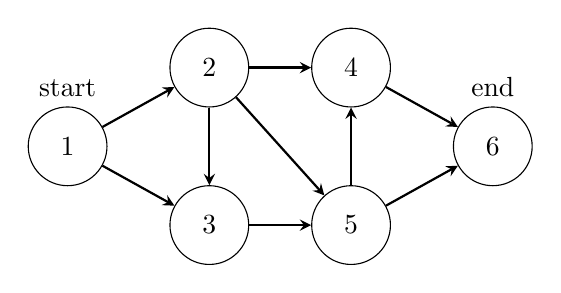
\begin{tikzpicture}[node distance = 1.8cm]
						\node (1) [circleNode, label=above:start] {1};
						\node (2) [circleNode, right of=1, yshift=1cm] {2};
						\node (3) [circleNode, right of=1, yshift=-1cm] {3};
						\node (4) [circleNode, right of=2] {4};
						\node (5) [circleNode, right of=3] {5};
						\node (6) [circleNode, label=above:end, right of=4, yshift=-1cm] {6};
						\draw [arrow] (1) -- (2);
						\draw [arrow] (1) -- (3);
						\draw [arrow] (2) -- (3);
						\draw [arrow] (2) -- (4);
						\draw [arrow] (3) -- (5);
						\draw [arrow] (4) -- (6);
						\draw [arrow] (5) -- (6);
						\draw [arrow] (5) -- (4);
						\draw [arrow] (2) -- (5);
					\end{tikzpicture}
					\caption{Example of directed graph}
				\end{figure}
				Denote:\\
				\begin{equation}
					x_{ij} = \begin{cases}1, &\text{if goes from } i \text{ to } j\\ 0, & \text{otherwise}\end{cases}
				\end{equation}
				The shortest path problem can be formulated as the following:\\
				\begin{align}
					\min &\sum_{(i, j)\in A} c_{ij}x_{ij} \\
					& \sum_{i \in N\setminus(\{S\}\cup\{E\}), (i,j)\in A} x_{ij} - \sum_{j \in N, (i,j)\in A} x_{ji} = 0 \\
					& \sum_{i=\{S\}, (i,j)\in A} x_{ij} - \sum_{j \in N, (i,j)\in A} x_{ji} = 1 \\
					& \sum_{i=\{E\}, (i,j)\in A} x_{ij} - \sum_{j \in N, (i,j)\in A} x_{ji} = -1 \\
					& x_{ij} \in [0,1], (i,j)\in A 
				\end{align}
				Although initially $x_{ij} \in [0,1]$, in the optimized solution, $x\in \{0, 1\}$.

			\subsection{Maximum Flow Problem}
				\begin{align}
					\min &\sum_{(i, j)\in A} F \\
					& \sum_{i \in N\setminus(\{S\}\cup\{E\}), (i,j)\in A} x_{ij} - \sum_{j \in N, (i,j)\in A} x_{ji} = 0 \\
					& \sum_{i=\{S\}, (i,j)\in A} x_{ij} - \sum_{j \in N, (i,j)\in A} x_{ji} = F \\
					& \sum_{i=\{E\}, (i,j)\in A} x_{ij} - \sum_{j \in N, (i,j)\in A} x_{ji} = -F \\
					& l_{ij} \le x_{ij} \le u_{ij}, (i,j)\in A 
				\end{align}
				In where $F$ means the flow from source to target.

			\subsection{Minimum Cost Flow}
				The shortest path problem is a special case of Minimum Cost Flow Problem, which can be formulated as the following:\\
				\begin{align}
					\min &\sum_{(i, j)\in A} c_{ij}x_{ij} \\
					& \sum_{i \in N\setminus(\{S\}\cup\{E\}), (i,j)\in A} x_{ij} - \sum_{j \in N, (i,j)\in A} x_{ji} = 0 \\
					& \sum_{i=\{S\}, (i,j)\in A} x_{ij} - \sum_{j \in N, (i,j)\in A} x_{ji} = 1 \\
					& \sum_{i=\{E\}, (i,j)\in A} x_{ij} - \sum_{j \in N, (i,j)\in A} x_{ji} = -1 \\
					& x_{ij} \in [0,1], (i,j)\in A 
				\end{align}				
			
			\subsection{Unimodularity}
				\subsubsection{Unimodular Matrix and Total Unimodular Matrix}
					- A unimodular matrix $M$ is a squared matrix, where $det(M)=1$ or $-1$.\\
					- Total unimodular matrix is a matrix where all its sub-matrices are unimodular matrix.

				\subsubsection{Importance of Unimodular Matrix}
					Let $M_{m\times m}$ be a unimodular matrix, if $b\in \mathbb{Z}^m$, the solution for $Mx=b$ is always integer.\\
					\framebox{\textbf{Proof:}} By Cramer's Rule
					\begin{equation}
						x_i = \frac{det{M_i}}{det{M}} 
					\end{equation}
					in which $M_i$ is matrix $M$ replace $i$th column with $b$. Therefore $det(M_i)$ is integer. Also, $det(M)\ne 0$, so $det(M)=1$ or $det(M)=-1$. Proved.

				\subsubsection{Structures of Total Unimodular Matrix}
					\textbf{Structure 1:}
						Matrix $M$ that has only 1, -1, 0 enters and each column has at most 2 non-zeros is a TU matrix if it satisfies the following conditions:\\
						We can split the rows in to tops and bottoms, such that for all columns $j$ having 2 non-zeros\\
						- If the non-zeros have the same sign, then one value should be in top and the other should be in bottom\\
						- If the non-zeros have the different sign, then both of them should be in top or both of them should be in bottom\\
					\textbf{Structure 2:}
						If all the columns in matrix $M$ has only 0 or consecutive 1s (or -1s), matrix $M$ is a TU matrix

				\subsubsection{Construct a New Unimodular Matrix}
					Let $F$ be a unimodular matrix, then
					\begin{equation}
						\left[\begin{matrix}F \\ I\end{matrix}\right] 
					\end{equation}
					is a unimodular matrix, also
					\begin{equation}
						\left[\begin{matrix}F & 0 \\ I & I\end{matrix}\right] 
					\end{equation}
					is a unimodular matrix.
	\part{Nonlinear Programming}
	\chapter{Introduction and Movtivation}
		\section{Basic concept}
			\begin{align}
				\min \quad &f(x) \\
				\text{s.t.} \quad & g_i(x) \le 0, \quad \forall i = 1, ..., m\\
								  & h_i(x) = 0, \quad \forall i = 1, ..., m\\
								  &x \in X
			\end{align}

			Iso-value curve\\
			Given a function $f(x): R^n \rightarrow R$, the iso-value curve of level k, denoted by $L_k$ is the set of points for which $f(x)=k$, Formally,
			\begin{equation}
				L_k = \{x \in R^n | f(x)=k\}
			\end{equation}

			Observations:\\
			\indent - An optimization problem may not have a feasible solution\\
			\indent - Even if the problem has a feasible solution, the problem may not have an optimal solution\\
			\indent - If an optimal solution exists, then\\
			\indent \indent - if may be unique
			\indent \indent - it may be a convex set
			\indent \indent - it may be serveral sets

			The following two problems are equivalent
			\begin{align}
				\min \quad & x_1 + x_2\\
				\text{s.t.} \quad & x_1 + 2x_2\le 3 \\
				                  & x_1, x_2 \in \{0, 1\}
			\end{align}
			and 
			\begin{align}
				\min \quad & x_1 + x_2\\
				\text{s.t.} \quad & x_1 + 2x_2\le 3 \\
				                  & x_1 \ge 0 \\
				                  & x_2 \ge 0 \\
				                  & x_1(1 - x_1) = 0\\
				                  & x_2(1 - x_2) = 0
			\end{align}		

			\section{Example - Braess Paradox}

			- Situation 1, minimizing total time
			\begin{align}
				\min \quad & \frac{x_1t_1 + x_2t_2 + x_3t_3}{x_1 + x_2 + x_3}\\
				\text{s.t.} \quad & x_1 + x_2 + x_3 = 1000\\
				                  & t_1 = 1 + (x_1 + x_2) / 1000 + 2\\
				                  & t_2 = 1 + (x_1 + x_2) / 1000 + 0.25 + (x_2 + x_3)/1000 + 1\\
				                  & t_3 = 2 + (x_2 + x_3) / 1000 + 1
			\end{align}

			- Situation 2, selfish for driver
			\begin{align}
				\text{s.t.} \quad & x_1 + x_2 + x_3 = 1000\\
				                  & t_1 = 1 + (x_1 + x_2) / 1000 + 2\\
				                  & t_2 = 1 + (x_1 + x_2) / 1000 + 0.25 + (x_2 + x_3)/1000 + 1\\
				                  & t_3 = 2 + (x_2 + x_3) / 1000 + 1\\
				                  & x_1 t_1 \le x_1 t_2 \\
				                  & x_1 t_1 \le x_1 t_3 \\
				                  & x_2 t_2 \le x_2 t_1 \\
				                  & x_2 t_2 \le x_2 t_3 \\
				                  & x_3 t_3 \le x_3 t_1 \\
				                  & x_3 t_3 \le x_3 t_2
			\end{align}

			- Situation 3, remove one of the arc, remove $x_2$ and all related constraints

		\section{Newsvendor problem}
			Parameter
			\begin{itemize}
				\item for each newspaper, cost is \$c
				\item vendor determine the number of newspaper to buy as $N$
				\item each news paper selled for \$p
				\item each news paper has a salvage value of \$v
				\item for demend scenario $d_i, i\in N$, the probability is $\pi_i \in N$
			\end{itemize}

			Decision Vars
			\begin{itemize}
				\item number of newspaper to buy, $q$
				\item number of newspaper returned, $r_i, i \in N$
				\item number of newspaper sold, $s_i, i\in N$
			\end{itemize}

			Constraints
			\begin{itemize}
				\item $q = s_i + r_i$
				\item $s_i = \min \{d_i, q\}$
				\item $q \in Z_+ \cup \{0\}$
				\item $r_i, s_i \in Z_+ \cup \{0\}$
			\end{itemize}

			Objective Fuction
			\begin{equation}
				\max \quad \sum_{i \in N} \pi_i (ps_i + vr_i) - cq
			\end{equation}

		\section{Portfolio optimization}
			Parameters
			\begin{itemize}
				\item A, set of assets
				\item $\bar{r}$, desired portfolio's return
				\item $r_i$, expected return of $i\in A$
				\item $\sigma_{ij}^2$, covariance between $i$ and $j$, $i, j \in A$
			\end{itemize}

			Decision Vars
			\begin{itemize}
				\item $x_i$ \% of total budget to invest to asset $i \in A$
			\end{itemize}

			Constraints
			\begin{itemize}
				\item $\sum_{i \in A} x_i = 1$
				\item $\sum_{i \in A} \alpha_i x_i \ge \bar{r}$
				\item Nonnegativity
			\end{itemize}

			Objective function
			\begin{equation}
				\min \quad \sum_{i \in A}\sum_{j \in A} \sigma_{ij}^2 x_i x_j
			\end{equation}

		\section{curve fitting}
			

	\chapter{KKT Optimality Conditions}

	\chapter{Lagrangian Duality}

	\chapter{Unconstrained Optimization}

	\chapter{Penalty and Barrier Functions}
	\part{Algorithms and Computational Complexity}
	\chapter{Computational Complexity}

	\chapter{Sorting}
		\section{Elementary Sorting Algorithms}

		\section{Heap-sort}

		\section{Quick-sort}

		\section{Sorting in Linear Time}

		\section{Medians and Order Statistics}

	\chapter{Data Structures}
		\section{Elementary Data Structures}

		\section{Hash Tables}

		\section{Binary Search Trees}

		\section{Red-Black Trees}

		\section{B-Trees}

		\section{Fibonacci Heaps}

		\section{van Emde Boas Trees}

	\chapter{Design and Analysis Techniques}
		\section{Dynamic Programming}

		\section{Greedy Algorithms}

		\section{Amortized Analysis}

		\section{Multi-threaded Algorithms}

		\section{Matrix Operations}

		\section{Polynomials and the FFT}

		\section{Number-Theoretic Algorithms}

		\section{String Matching}

		\section{Computational Geometry}

		\section{NP-Completeness}

		\section{Approximation Algorithms}

	\part{Heuristics ans Meta-heuristics}
	\part{Game Theory}
	\chapter{Games with Ordinal Payoffs}
		\section{Ordinal Games in Strategic Form}

		\section{Perfect-information Games}

		\section{General Dynamic Games}

	\chapter{Games with Cardinal Payoffs}
		\section{Expected Utility Theory}

		\section{Strategic-form Games}

		\section{Extensive-form Games}

	\chapter{Knowledge, Common Knowledge, Beliefs}
		\section{Common Knowledge}

		\section{Adding Beliefs to Knowledge}

		\section{Rationality}

	\chapter{Refinements of Subgame-perfect Equilibrium}
		\section{Weak Sequential Equilibrium}

		\section{Sequential Equilibrium}

		\section{Perfect Bayesian Equilibrium}

	\chapter{Incomplete Information}
		\section{Static Games}

		\section{Dynamic Games}

		\section{The Type-Space Approach}
	\part{Probability, Stochastic Processes and Markov Chains}
	\chapter{Probability}

	\chapter{Random Variables}
		\section{Relationship between Some Random Variables}
			\begin{figure}[h]
				\centering
				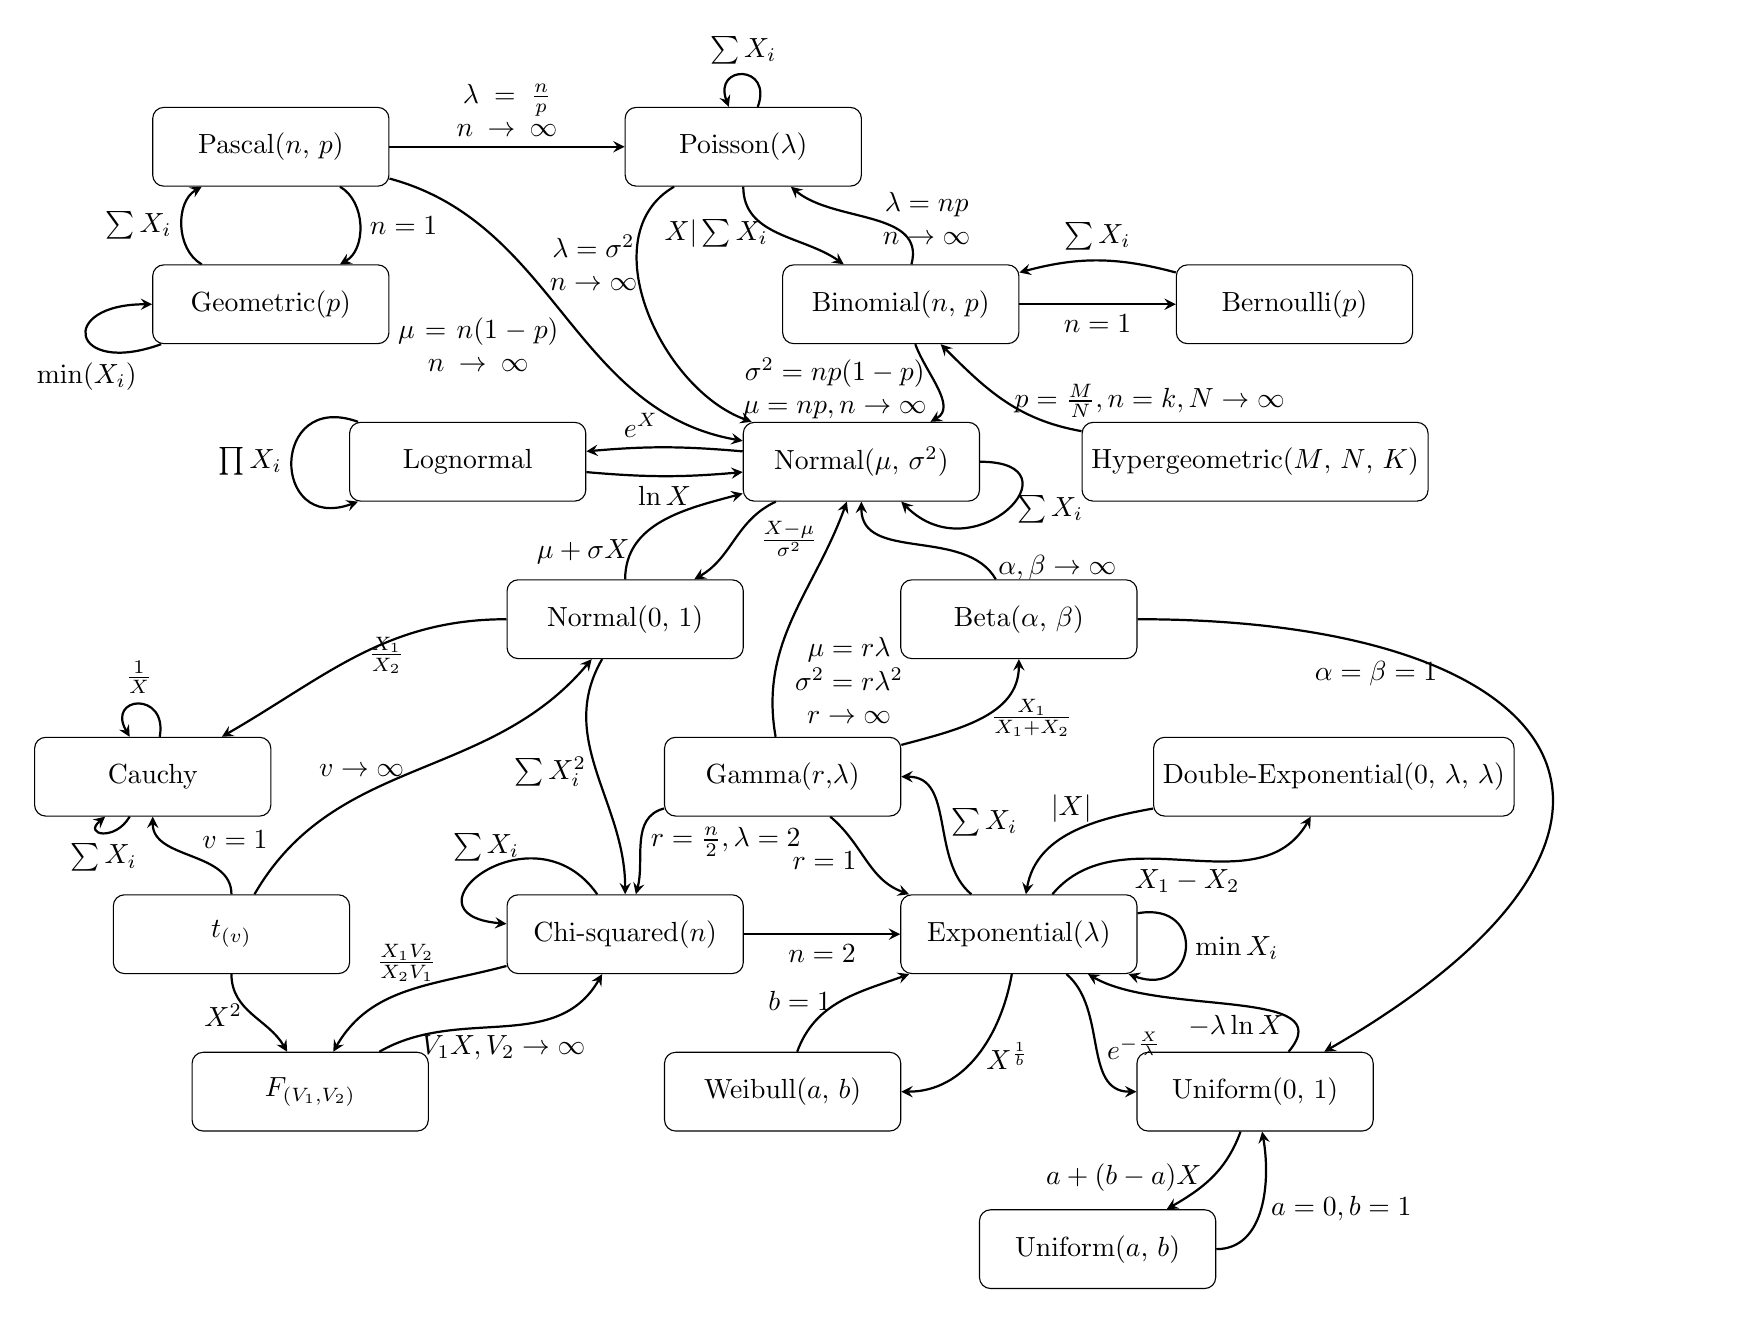
\begin{tikzpicture}[node distance = 2cm]
					\node (Pascal) [roundedRectangle] {Pascal($n$, $p$)};
					\node (Poisson) [roundedRectangle, xshift = 6cm] {Poisson($\lambda$)};
					\node (Geometric) [roundedRectangle, below of = Pascal] {Geometric($p$)};
					\node (Binomial) [roundedRectangle, below of = Poisson, xshift = 2cm] {Binomial($n$, $p$)};
					\node (Bernoulli) [roundedRectangle, below of = Poisson, xshift = 7cm] {Bernoulli($p$)};
					\node (Lognormal) [roundedRectangle, below of = Geometric, xshift = 2.5cm] {Lognormal};
					\node (Normal) [roundedRectangle, below of = Geometric, xshift = 7.5cm] {Normal($\mu$, $\sigma^2$)};
					\node (Hypergeometric) [roundedRectangle, below of = Geometric, xshift = 12.5cm] {Hypergeometric($M$, $N$, $K$)};
					\node (SNormal) [roundedRectangle, below of = Lognormal, xshift=2cm] {Normal(0, 1)};
					\node (Beta) [roundedRectangle, below of = Lognormal, xshift = 7cm] {Beta($\alpha$, $\beta$)};
					\node (DExponential) [roundedRectangle, below of = Beta, xshift = 4cm] {Double-Exponential($0$, $\lambda$, $\lambda$)};
					\node (Cauchy) [roundedRectangle, below of = SNormal, xshift = -6cm] {Cauchy};
					\node (Gamma) [roundedRectangle, below of = SNormal, xshift = 2cm] {Gamma($r$,$\lambda$)};
					\node (tv) [roundedRectangle, below of = Cauchy, xshift = 1cm] {$t_{(v)}$};
					\node (Chi-squared) [roundedRectangle, below of = Gamma, xshift = -2cm] {Chi-squared($n$)};
					\node (Exponential) [roundedRectangle, below of = Gamma, xshift = 3cm] {Exponential($\lambda$)};
					\node (Fvv) [roundedRectangle, below of = tv, xshift = 1cm] {$F_{(V_{1},V_{2})}$};
					\node (Weibull) [roundedRectangle, below of = Exponential, xshift = -3cm] {Weibull($a$, $b$)};
					\node (SUniform) [roundedRectangle, below of = Exponential, xshift = 3cm] {Uniform($0$, $1$)};
					\node (Uniform) [roundedRectangle, below of = SUniform, xshift = -2cm] {Uniform($a$, $b$)};
					\draw [arrow] (Pascal) to [out = -30, in = 30] node [right] {$n=1$} (Geometric);
					\draw [arrow] (Pascal) -- node [above, align=center, text width=2.5cm] {$\lambda=\frac{n}{p}$ \\ $n\rightarrow \infty$} (Poisson);
					\draw [arrow] (Pascal) to [out = -15, in = 170] node [below, align=center, text width=2.5cm, yshift=0.1cm, xshift=-1.1cm] {$\mu = n(1-p)$ \\ $n\rightarrow \infty$} (Normal);
					\draw [arrow] (Geometric) to [out = 150, in = -150] node [left] {$\sum X_i$} (Pascal);
					\draw [arrow] (Geometric) to [out = -160, in = 180, looseness=6] node [below, yshift = -0.2cm] {$\min(X_i)$} (Geometric);
					\draw [arrow] (Poisson) to [out = 70, in = 110, looseness=4] node [above] {$\sum X_i$} (Poisson);
					\draw [arrow] (Poisson) to [out = -90, in = 145] node [left] {$X|\sum X_i$} (Binomial);
					\draw [arrow] (Poisson) to [out = -150,in = 160] node [left, align=center, yshift=0.6cm] {$\lambda=\sigma^2$ \\ $n\rightarrow \infty$} (Normal);
					\draw [arrow] (Binomial) to [out = 75, in = -40] node [right, align=center] {$\lambda=np$ \\ $n\rightarrow \infty$} (Poisson);
					\draw [arrow] (Binomial) -- node [below] {$n=1$} (Bernoulli);
					\draw [arrow] (Bernoulli) to [out = 165, in = 15] node [above] {$\sum X_i$} (Binomial);
					\draw [arrow] (Binomial) to [out = -70, in = 30, align=center] node [left] {$\sigma^2=np(1-p)$ \\ $\mu=np, n\rightarrow \infty$} (Normal);
					\draw [arrow] (Hypergeometric) to [out = 170, in = -45] node [right] {$p=\frac{M}{N}, n=k, N\rightarrow \infty$} (Binomial);
					\draw [arrow] (Normal) to [out = 0, in = -45, looseness=3] node [right] {$\sum X_i$} (Normal);
					\draw [arrow] (Normal) to [out = 175, in = 5] node [above, xshift=-0.3cm] {$e^{X}$} (Lognormal);
					\draw [arrow] (Normal) to [out = -155, in = 30] node [right, xshift=0.2cm] {$\frac{X-\mu}{\sigma^2}$} (SNormal); 
					\draw [arrow] (Lognormal) to [out = -5, in = -175] node [below] {$\ln X$} (Normal);
					\draw [arrow] (Lognormal) to [out = 160, in = -160, looseness = 3] node [left] {$\prod X_i$} (Lognormal);
					\draw [arrow] (SNormal) to [out = 90, in = -165] node [left, yshift = -0.4cm, xshift = -0.3cm] {$\mu + \sigma X$} (Normal);
					\draw [arrow] (Beta) to [out = 120, in = -90] node [right, yshift=-0.3cm, xshift=0.9cm] {$\alpha, \beta \rightarrow \infty$} (Normal);
					\draw [arrow] (Beta) to [out = 0, in = 30, looseness=2.4] node [right, yshift=1cm, xshift=-3cm] {$\alpha=\beta=1$} (SUniform);
					\draw [arrow] (Gamma) to [out = 100, in = -110] node [right, align = center, yshift=-0.8cm, xshift = -0.1cm] {$\mu=r\lambda$\\$\sigma^2=r\lambda^2$\\$r\rightarrow \infty$} (Normal); 
					\draw [arrow] (Gamma) to [out = 15, in = -90] node [right] {$\frac{X_1}{X_1 + X_2}$} (Beta);
					\draw [arrow] (Gamma) to [out = -165, in = 75] node [right] {$r=\frac{n}{2}, \lambda=2$} (Chi-squared);
					\draw [arrow] (Gamma) to [out = -40, in = 160] node [left] {$r=1$} (Exponential);
					\draw [arrow] (SNormal) to [out = 180, in = 30] node [right] {$\frac{X_1}{X_2}$} (Cauchy);
					\draw [arrow] (SNormal) to [out = -120, in =90] node [left] {$\sum X_i^2$} (Chi-squared);
					\draw [arrow] (Cauchy) to [out = 80, in = 120, looseness = 4] node [above] {$\frac{1}{X}$} (Cauchy);
					\draw [arrow] (Cauchy) to [out = -120, in = -140, looseness = 3] node [below] {$\sum X_i$} (Cauchy);
					\draw [arrow] (tv) to [out = 90, in = -90] node [right, yshift = 0.2cm] {$v=1$} (Cauchy);
					\draw [arrow] (tv) to [out = 60, in = -130] node [left] {$v\rightarrow \infty$} (SNormal);
					\draw [arrow] (tv) to [out = -90, in = 120] node [left] {$X^2$} (Fvv);
					\draw [arrow] (Fvv) to [out = 30, in = -120] node [below] {$V_1X, V_2\rightarrow \infty$} (Chi-squared);
					\draw [arrow] (Chi-squared) to [out = -165, in = 60] node [above] {$\frac{X_1V_2}{X_2V_1}$} (Fvv);
					\draw [arrow] (Chi-squared) to [out = 125, in = 175, looseness = 3] node [above] {$\sum X_i$} (Chi-squared);
					\draw [arrow] (Chi-squared) -- node [below] {$n=2$} (Exponential);
					\draw [arrow] (Exponential) to [out = 140, in = 0] node [right] {$\sum X_i$} (Gamma);
					\draw [arrow] (Exponential) to [out = 50, in = -120] node [below] {$X_1 - X_2$} (DExponential);
					\draw [arrow] (Exponential) to [out = 10, in = -20, looseness = 3] node [right] {$\min X_i$} (Exponential);
					\draw [arrow] (Exponential) to [out = -40, in = 180] node [right] {$e^{-\frac{X}{\lambda}}$} (SUniform);
					\draw [arrow] (Exponential) to [out = -100, in = 0] node[right] {$X^{\frac{1}{b}}$} (Weibull);
					\draw [arrow] (DExponential) to [out = -170, in = 80] node [above] {$|X|$} (Exponential);
					\draw [arrow] (Uniform) to [out = 0, in = -80] node [right] {$a=0, b=1$} (SUniform);
					\draw [arrow] (SUniform) to [out = 50, in = -30] node [below] {$-\lambda \ln X$} (Exponential);
					\draw [arrow] (SUniform) to [out = -110, in = 30] node [left] {$a+(b-a)X$} (Uniform);
					\draw [arrow] (Weibull) to [out = 70, in = -160] node [left] {$b=1$} (Exponential);
				\end{tikzpicture}
				\caption{Relationship between Some Random Variables}
			\end{figure}

		\begin{landscape}
		\section{Discrete Random Variables}
			\begin{longtable}[c]{|c|c|c|c|c|c|}
				\caption{Discrete Random Variables \label{DRV}}\\
				\hline
				Distribution & PMF & CDF & Expectation & Variance & MGF \\
				\hline
				\endfirsthead
				\hline
				Distribution & PMF & CDF & Expectation & Variance & MGF \\
				\hline
				\endhead
				Discrete Uniform$(a, b)$ & 
				\makecell{$f(x)=\frac1{b-a+1}$ \\ $x=a, a+1, ..., b$} & 
				\makecell{$F(x)=\frac{x-a+1}{b-a+1}$ \\ $x=a, a+1, ..., b$} & 
				$E[X]=\frac{b-a}{2}$ & 
				$D[X]=\frac{(b-a+1)^2-1}{12}$ & 
				\makecell{$M(t)=\frac{e^{at}-e^{(b+1)t}}{(b-a+1)(1-e^t)}$ \\ $t \in \mathbb{R}$} \\
				\hline
				Bernoulli$(p)$ & 
				\makecell{$f(x)=p^x(1-p)^{1-x}$ \\ $x \in \{0,1\}$} &
				$F(x)=\begin{cases}0, \quad x<0 \\ 
									1-p, \quad 0\le x \le 1 \\
									1, \quad x>1\end{cases}$ & 
				$E[X]=p$ & 
				$D[X]=p(1-p)$ & 
				\makecell{$M(t)=1-p+pe^{t}$ \\ $t\in \mathbb{R}$}\\
				\hline
				Binomial$(n, p)$ &
				\makecell{$f(x)=\left(\begin{matrix}n\\x\end{matrix}\right)p^x(1-p)^{n-x}$ \\ $x=0,1,...,n$} &
				\makecell{$F(x)=\sum_{k=0}^{x}\left(\begin{matrix}n\\k\end{matrix}\right)p^k(1-p)^{n-k}$ \\ $x=0,1,...,n$} &
				$E[X]=np$ &
				$D[X]=np(1-p)$ &
				\makecell{$M(t)=(1-p+pe^{t})^n$ \\ $t\in \mathbb{R}$}\\
				\hline
				Poisson$(\mu)$ &
				\makecell{$f(x)=\frac{\mu^xe^\mu}{x!}$ \\ $x = 0,1,...,n,...$} &
				\makecell{$f(x)=\frac{\Gamma(x+1, \mu)}{\Gamma(x+1)}$ \\ $x=0,1,...,n,...$} &
				$E[X]=\mu$ &
				$D[X]=\mu$ &
				\makecell{$M(t)=e^{\mu(e^t-1)}$ \\ $t\in \mathbb{R}$} \\
				\hline
				Geometric$(p)$ &
				\makecell{$f(x)=p(1-p)^x$ \\ $x=0,1,...,n,...$} &
				\makecell{$F(x)=1-(1-p)^{x+1}$ \\ $x=0,1,...,n,...$} &
				$E[X]=\frac{1-p}p$ &
				$D[X]=\frac{1-p}{p^2}$ &
				\makecell{$M(t)=\frac{p}{1-(1-p)e^t}$ \\ $t < -\ln(1-p)$}\\
				\hline
				Pascal$(n, p)$ &
				\makecell{$f(x)=\left(\begin{matrix}n-1+x\\x\end{matrix}\right)p^n(1-p)^x$ \\ $x=0,1,2,...,n,...$} &
				\makecell{$F(x)=1-I_p(k+1,n)$ \\ $x=0,1,2,...,n,...$} &
				$E[X]=\frac{n(1-p)}{p}$&
				$D[X]=\frac{n(1-p)}{p^2}$ &
				\makecell{$M(t)=(\frac{p}{1-(1-p)e^t})^n$ \\ $t < -\ln(1-p)$}\\
				\hline
			\end{longtable}

		\section{Continuous Random Variables}
			\begin{longtable}[c]{|c|c|c|c|c|c|}
				\caption{Continuous Random Variables \label{CRV}}\\
				\hline
				Distribution & PDF & CDF & Expectation & Variance & MGF \\
				\hline
				\endfirsthead
				\hline
				Distribution & PDF & CDF & Expectation & Variance & MGF \\
				\hline
				\endhead
				Uniform$(a, b)$ & 
				\makecell{$f(x)=\frac1{b-a}$ \\ $x=[a,b]$} & 
				\makecell{$F(x)=\frac{x-a}{b-a}$ \\ $x=[a,b]$} & 
				$E[X]=\frac{b-a}{2}$ & 
				$D[X]=\frac{(b-a)^2}{12}$ & 
				$M(t)=\begin{cases}1, \quad t=0 \\ \frac{e^{bt}-e^{at}}{t(b-a)}, \quad t\ne 0\end{cases}$\\
				\hline
				Normal$(\mu, \sigma)$ &
				\makecell{$f(x)=\frac{1}{\sqrt{2\pi}\sigma}e^{-\frac{(x-\mu)^2}{2\sigma^2}}$ \\ $x\in \mathbb{R}$} &
				\makecell{$F(x)=\int_{-\infty}^{x}\frac{1}{\sqrt{2\pi}\sigma}e^{-\frac{(x-\mu)^2}{2\sigma^2}}$ \\ $x\in \mathbb{R}$} &
				$E[X]=\mu$ &
				$D[X]=\sigma^2$ &
				\makecell{$e^{\frac{t(t\sigma^2+2\mu)}{2}}$ \\ $t\in \mathbb{R}$}\\
				\hline
				Exponential$\lambda)$ &
				\makecell{$f(x)=\lambda e^{-\lambda x}$ \\ $x>0$} &
				\makecell{$F(x)=1-e^{\lambda x}$ \\ $x>0$} &
				$E[X]=\frac{1}{\lambda}$ &
				$D[X]=\frac{1}{\lambda^2}$ &
				\makecell{$\frac{1}{1-\frac{t}{\lambda}}$ \\ $t<\lambda$}\\
				\hline
				Erlang$(n, \lambda)$ &
				\makecell{$f(x)=\frac{\lambda^n x^{n-1} e^{-\lambda x}}{(n-1)!}$ \\ $x>0$} &
				\makecell{$F(x)=1-\sum_{i=0}^{n-1}\frac{\lambda^n x^n e^{-\lambda x}}{n!}$ \\ $x>0$} &
				$E[X]=\frac{n}{\lambda}$ &
				$D[X]=\frac{n}{\lambda^2}$ &
				\makecell{$\frac{1}{(1-\frac{t}{\lambda})^n}$ \\ $t<\lambda$} \\
				\hline
			\end{longtable} 
		\end{landscape}

	\chapter{Limit Theorems}

	\chapter{The Bernoulli and Poisson Process}

	\chapter{Discrete-Time Markov Chains}

	\chapter{Continuous-Time Markov Chains}
	\part{Queuing Theory}
	\chapter{Queuing Model}

	\chapter{Birth-and-Death Queuing Models}

	\chapter{Multidimensional Birth-and-Death Queuing Models}

	\chapter{Phase-Type Queue}

	\chapter{Bulk Queue}

	\chapter{Imbedded-Markov-Chain Queuing Models}

	\chapter{Queuing Network}
	\part{Inventory Theory}
	\part{Reliability Theory}
	\part{Statistic}
	\part{Simulation}
\end{document}